%%% File encoding: UTF-8
%%% äöüÄÖÜß  <-- keine deutschen Umlaute hier? UTF-faehigen Editor verwenden!

%%% Magic Comments zum Setzen der korrekten Parameter in kompatiblen IDEs
% !TeX encoding = utf8
% !TeX program = pdflatex 
% !TeX spellcheck = de_DE
% !BIB program = biber

\documentclass[master,german]{hgbthesis}
% Zulässige Optionen in [..]: 
%   Typ der Arbeit: diploma, master (default), bachelor, internship
%   Hauptsprache: german (default), english
%		smartquotes: zur vereinfachten Eingabe von Hochkommas (nur "...")
%%%----------------------------------------------------------

\RequirePackage[utf8]{inputenc}		% bei der Verw. von lualatex oder xelatex entfernen!
\RequirePackage{multirow}

\graphicspath{{images/}}    % Verzeichnis mit Bildern und Grafiken
\logofile{logo}							% Logo-Datei = images/logo.pdf (\logofile{}, wenn kein Logo gewünscht)
\bibliography{references}  	% Biblatex-Literaturdatei (references.bib)

%%%----------------------------------------------------------
% Angaben für die Titelei (Titelseite, Erklärung etc.)
%%%----------------------------------------------------------

%%% Einträge für ALLE Arbeiten: -----------------------------
\title{MiniJava-Compiler für WebAssembly auf Basis von ANTLR und Kotlin}
\author{Stefan Schöberl, BSc}

\programtype{Fachhochschul-Masterstudiengang}

\programname{Software Engineering}
\placeofstudy{Hagenberg}
\dateofsubmission{2020}{06}{30}	% {YYYY}{MM}{DD}

\advisor{FH-Prof. DI Dr. Heinz Dobler}	% optional

%\strictlicense		%%% restrictive license instead of Creative Commons (discouraged!)

\RequirePackage{hyphenation}

%%%----------------------------------------------------------
\begin{document}
%%%----------------------------------------------------------

\setlength{\parindent}{0pt}
\setlength{\parskip}{0.5em}

%%%----------------------------------------------------------
\frontmatter                    % Titelei (röm. Seitenzahlen)
%%%----------------------------------------------------------

\maketitle

\chapter{Kurzfassung}

WebAssembly ist eine neue Technologie, die mittlerweile in aktuellen Browsern integriert ist. Seit Dezember 2019 ist WebAssembly ein offizieller Web"=Stanard des W3C. WebAssembly verwendet einen eigenen Bytecode, dessen Ausführungsmodell auf einer virtuellen Kellermaschine basiert und verspricht schnellere Ladezeiten und bessere Performanz als beispielsweise JavaScript. Dadurch ist es möglich, andere Programmiersprachen ohne Transpiler im Web einzusetzen. Dafür sind allerdings Compiler notwendig, die für WebAssembly Bytecode erzeugen können. Java Applets verfolgten einen ähnlichen Ansatz, indem sie die Java Virtual Machine (JVM) im Browser einsetzten, jedoch wird diese Technologie mittlerweile nicht mehr in aktuellen Browsern unterstützt.

Diese Masterarbeit befasst sich mit der Entwicklung eines Compilers für MiniJava, einer Teilmenge der von Java. Dabei wird gezeigt, wie Sprachkonstrukte dieser Programmiersprache auf WebAssembly abgebildet werden können. Weiters wird auf das zur Ausführung notwendige Laufzeitsystem eingegangen. Eine Besonderheit dabei ist, dass Objekte in MiniJava auf JavaScript"=Objekte abgebildet werden, dadurch ist beispielsweise im Browser ein direkter DOM"=Zugriff möglich. Die praktische Anwendung des geschaffenen Compilers wird anhand einer Demo"=Anwendung im Browser, einem Fibonacci"=Rechner, demonstriert. Diese Anwendung wurde, bis auf generische notwendige Skripte zum Laden der Anwendung, zur Gänze in MiniJava implementiert.

In dieser Masterarbeit wird damit eine Möglichkeit aufgezeigt, wie neue Programmiersprachen auf Basis von WebAssembly in das Web gebracht werden können.

\chapter{Abstract}


\begin{english}
WebAssembly is a new technology, which is supported in current browsers by now. Since december 2019 WebAssembly is an official Web standard of the W3C. Web\-As\-sem\-bly uses its own bytcode, whose execution model is based on a stack machine and promises faster loading times and better performance than JavaScript, for example. Thus it is possible, to bring other programming languages without a transpiler to the Web. However, compilers are necessary, that can produce bytecode for WebAssembly. Java Applets were based on a similar approach by using the Java virtual machine (JVM) within the browser, but this technology is no longer supported in current browsers.

This master's thesis deals with the development of a compiler for MiniJava, a subset of Java. It is shown how features of this programming language will be mapped to WebAssembly. In addition, the runtime system required for execution is described. A special feature is the direct mapping of objects in MiniJava to JavaScript objects. This enables direct DOM access in the browser, for example. The practical use of the created compiler is demonstrated with a browser demo application, which is a Fibonacci calculator. This application was implemented entirely in MiniJava, except for some generic scripts required to load the application.

This master's thesis shows an approach, how new programming languages can be brought to the Web based on WebAssembly.
\end{english}


\tableofcontents

\chapter{Vorwort und Dank}
 
Compiler und die Hintergründe von Programmiersprachen faszinieren mich schon seit langer Zeit. Mein Interesse vertiefte sich durch die Programmierlehranverstaltungen im Bachelorstudium und im Masterstudium durch die Lehrveranstaltung \emph{formale Sprachen, Compiler- und Werkzeugbau}, sodass für mich eine Masterarbeit in diesem Themenumfeld in Frage gekommen ist. Aus einem Vorschlag von Heinz Dobler zu \emph{WebAssembly} entstand so die Idee, mich mit dieser vielversprechenden neuen Technologie auseinanderzusetzen und einen Compiler für eine eigene Programmiersprache zu entwickeln.

Da ich bisher einiges an Erfahrung im Java"=Umfeld mit Kotlin gesammelt habe, wäre es naheliegend gewesen, einen Compiler für Kotlin zu entwickeln. Da die Stärken von Kotlin allerdings eher in der kompakten Ausdrucksweise liegen, die zwar für Kotlin"=ProgrammierInnen vorteilhaft ist, für CompilerbauerInnen allerdings einen Mehraufwand mit sich bringt, fiel die Wahl sehr schnell auf Java. Da Java allerdings (für eine Masterarbeit) immer noch viel zu umfangreich ist, unterstützt mein Compiler nur eine \emph{kleine} Teilmenge der Sprache: \emph{MiniJava}.

Ganz besonders möchte ich mich bei meinem Betreuer Heinz Dobler bedanken, der mich über den gesamten Entstehungsprozess stets unterstützt hat. Die interessanten Diskussionen und das wertvolle konstruktive Feedback habe ich immer sehr geschätzt! Außerdem möchte ich mich bei meiner Schwester Nicole Schöberl und meinem Studienkollegen Florian Guld bedanken, die meine Arbeit Korrektur gelesen haben.

Ich möchte mich besonders auch bei meiner Familie und bei allen bedanken, die mich unterstützt haben.


%%%----------------------------------------------------------
\mainmatter          % Hauptteil (ab hier arab. Seitenzahlen)
%%%----------------------------------------------------------

\chapter{Einleitung}

\section{Motivation}

WebAssembly \cite{WebAssemblyWebsite} ist eine relativ neue (2017) Technologie mit dem Ziel, eine sprachunabhängige Plattform fürs Web zu schaffen. Da nur JavaScript von Browsern unterstützt wird, ist man auf diese Sprache beschränkt. Früher konnte man auch Java-Applets mit Java entwickeln, die direkt im Browser ausgeführt werden konnten. Aktuelle Browserversionen unterstützen diese Technologie mittlerweile nicht mehr und Oracle stellt ebenfalls die Unterstützung ein \cite{OracleJavaSESupportRoadmap}.

Anders sieht es bei Sprachen wie beispielsweise TypeScript aus: Um diese im Browser auszuführen, muss der Quelltext zunächst mit einem Transpiler nach JavaScript übersetzt werden. Anschließend muss der resultierende JavaScript-Quelltext vom Browser zur Laufzeit interpretiert werden \cite{TypeScript}.

WebAssembly verfolgt einen alternativen Ansatz, in dem eine Laufzeitumgebung in Form eines Kellerautomaten vom Browser zur Verfügung gestellt wird, so ähnlich wie früher die Java Virtual Machine mit Java-Applets. Über eine JavaScript-Schnittstelle können zur Laufzeit Module geladen werden, die im Kellerautomat ausgeführt werden. Module müssen in Form eines eigenen Bytecodes zur Verfügung stehen.

Ein geeigneter Compiler kann nun eine (beliebige) Programmiersprache in diesen Bytecode übersetzen. So ist ein Konvertieren des Quelltextes über einen Transpiler nicht mehr notwendig.

WebAssembly ist nicht als Alternative, sondern als Ergänzung zu JavaScript zu sehen. Ein Ziel ist, bestehenden Quelltext wiederverwenden zu können, auch wenn dieser in einer anderen Programmiersprache geschrieben wurde. Mit JavaScript werden die einzelnen Komponenten anschließend miteinander verbunden.

Damit dieses Ziel erreicht werden kann, müssen Compiler verschiedener Sprachen in der Lage sein, WebAssembly-Bytecode zu erzeugen.

\section{Problemstellung}

Die Problemstellung für diese Masterarbeit lässt sich in folgende Fragen aufteilen:

\begin{enumerate}
	\item Was ist WebAssembly, welche Möglichkeiten bietet WebAssembly und welche Einschränkungen gibt es?
	\item Wie kann ein Compiler, der eine Programmiersprache nach WebAssembly übersetzt, implementiert und getestet werden?
	\item Wie werden typische Sprachkonstrukte einer Programmiersprache auf Web\-As\-sem\-bly-Befehle abgebildet?
	\item Wie wird die Schnittstelle zum Browser entworfen und auf welche Aspekte muss dabei geachtet werden?
\end{enumerate}

\section{Ziele}

Die Fragen der Problemstellung sollen auf auf Basis einer praktischen Implementierung beantwortet werden.

Ziel ist es, einen Compiler zu entwickeln, der MiniJava (eine Teilmenge von Java) nach WebAssembly übersetzt. Die Eingabe ist MiniJava-Quelltext, die Ausgabe ein WebAssembly-Modul samt Laufzeitsystem für JavaScript. Der gesamte Compiler wird in Kotlin entwickelt. Das Compiler-Frontend (Scanner und Parser) wird mit ANTLR 4 generiert.

Schlussendlich soll es möglich sein, in MiniJava eine kleine typische Web-Anwendung zu entwickeln.

Weiters wird eine minimale Standardbibliothek entworfen. Diese stellt essentielle Schnittstellen für die Konsole und den DOM-Zugriff zur Verfügung.

Es gibt bereits einige Technologien, die auf WebAssembly aufbauen. Auf drei ausgewählte wird in dieser Arbeit kurz eingangen:
\begin{itemize}
    \item Emscripten \cite{Emscripten} für C und C++
    \item Rust \cite{RustWasmWebsite}
    \item Blazor \cite{Blazor} 
\end{itemize}

Beim Einsatz von Emscripten und Rust ist im C/C++/Rust-Quelltext ersichtlich, dass JavaScript oder WebAssembly im Hintergrund verwendet wird. Bei Emscripten sind das beispielsweise Einschlüsse von JavaScript-Fragmenten oder bei Rust müssen spezielle Attribute eingefügt werden. Blazor ist ein Framework zum Entwickeln von Web-Anwendungen und bietet somit eine Komplettlösung an. Hier kann bestehender C\#{}-Code unter gewissen Voraussetzungen wiederverwendet werden.

Mit MiniJava soll ein alternativer Ansatz versucht werden, eine (neue) Programmiersprache ins Web über WebAssembly zu bringen: MiniJava-Quelltext soll im Unterschied zu Emscripten und Rust keine Hinweise darauf enthalten, dass der kompilierte Quelltext schlussendlich mit JavaScript und WebAssembly interagiert. Es soll mit MiniJava auch kein Framework aufgebaut werden wie bei Blazor. Weiters sollen Objekte in MiniJava 1:1 auf JavaScript-Objekte abgebildet werden, dadurch soll beispielsweise direkter Zugriff auf den DOM ermöglicht werden. Dieser Ansatz findet sich so in keiner der drei Technologien. Schnittstellen zur Laufzeitumgebung werden in MiniJava über native Methoden umgesetzt. Dieses Sprachkonstrukt ist aus Java bekannt.

\section{Aufbau der Arbeit}

Die Arbeit ist in aufeinander aufbauende Kapitel gegliedert:
\begin{enumerate}
    \setcounter{enumi}{1}
    \item \emph{Technische Grundlagen:} Die Implementierung dieser Arbeit baut auf diversen Technologien auf. In diesem Kapitel werden die für diese Arbeit notwendigen Technologien beschrieben. Ein besonderer Fokus liegt hier auf WebAssembly und ANTLR, es wird aber auch auf diverse Hilfstechnologien eingegangen. Zum Schluss werden drei aktuelle Technologien im Detail betrachtet, die bereits WebAssembly-Unterstützung anbieten.
    \item \emph{Anforderungen an den Compiler und das Laufzeitsystem:} In diesem Kapitel wird die Programmiersprache MiniJava vorgestellt. Dieses Kapitel ist als Art Anforderungskatalog für den Compiler und das Laufzeitsystem zu sehen.
    \item \emph{Codegenerierung für WebAssembly:} In diesem Kapitel wird gezeigt, wie aus Mi\-ni\-Ja\-va-Quell\-text ein WebAssembly-Modul erzeugt wird. Dabei wird insbesonders gezeigt, wie die Sprachkonstrukte auf WebAssembly abgebildet werden. 
    \item \emph{Integration mit JavaScript:} Das erzeugte WebAssembly-Modul benötigt zur Ausführung noch ein Laufzeitsystem, auf dieses wird in diesem Kapitel eingangen. Das Laufzeitsystem ist in JavaScript implementiert. Weiters wird vom Compiler auch JavaScript-Quelltext generiert, um das Modul ausführen zu können.
    \item \emph{Testen des Compilers und Integration des Compilers in Gradle:} Um eine korrekte Funktion des Compilers zu gewährleisten, muss er getestet werden. Auf diesen Aspekt wird in diesem Kapitel im Detail eingangen. Weiters wird gezeigt, wie der Compiler in Gradle integriert werden kann, um ihn so in eigenen Projekten verwenden zu können. Diese Integration wird anhand einer Konsolenanwendung veranschaulicht.
    \item \emph{Demo-Anwendungen im Browser:} In diesem Kapitel wird ein Fibonacci-Rechner als Web-Anwendung präsentiert, um die praktische Anwendung von MiniJava zu demonstrieren. Weiters wird hier kurz auf die Standardbibliothek für DOM-Zugriffe eingangen.
\end{enumerate}

Zum Schluss werden die Ergebnisse der Arbeit zusammengefasst und es wird ein Ausblick auf mögliche Erweiterungen gegeben.

\pagebreak
\section{Architektur des Gesamtsystems}

Um zu Beginn einen Überblick zu geben, wird in Abbildung \ref{fig:architecture} die Architektur des Gesamtsystems dargestellt. Nachfolgend werden die wichtigsten Vorgänge beschrieben:

\begin{enumerate}
    \item Die Eingaben des Compilers sind MiniJava- und Ja\-va\-Script-Quelltexte. Die Ja\-va\-Script-Quelltexte enthalten die Implementierung nativer Methoden.
    \item Die MiniJava-Quelltexte werden vom generierten Scanner und Parser analysiert und in Syntaxbäume umgewandelt. Diese Syntaxbäume werden mit \emph{Visitors} und Codegeneratoren zu einem WebAssembly-Modul (als Datenstruktur im Arbeitsspeicher) verarbeitet. Dabei werden ebenfalls Metainformationen über den Mi\-ni\-Ja\-va-Quelltext gesammelt.
    \item Der Paketgenerator erzeugt aus dem Modul, den Meta-Informationen und den JavaScript-Quelltexten ein Paket. Ein Paket ist ein Verzeichnis mit einer definierten Struktur. Darin ist unter anderem das WebAssembly-Modul als Datei enthalten.
    \item Das Laufzeitsystem lädt in der Laufzeitumgebung das Paket, dabei wird die Web\-As\-sem\-bly-API eingesetzt. Daraus entsteht ein lauffähiges Modul.
    \item Nun kann das Modul gestartet werden und Ausgaben auf der Konsole oder visuell im DOM erzeugen.
\end{enumerate}


\begin{figure}[]
    \centering
    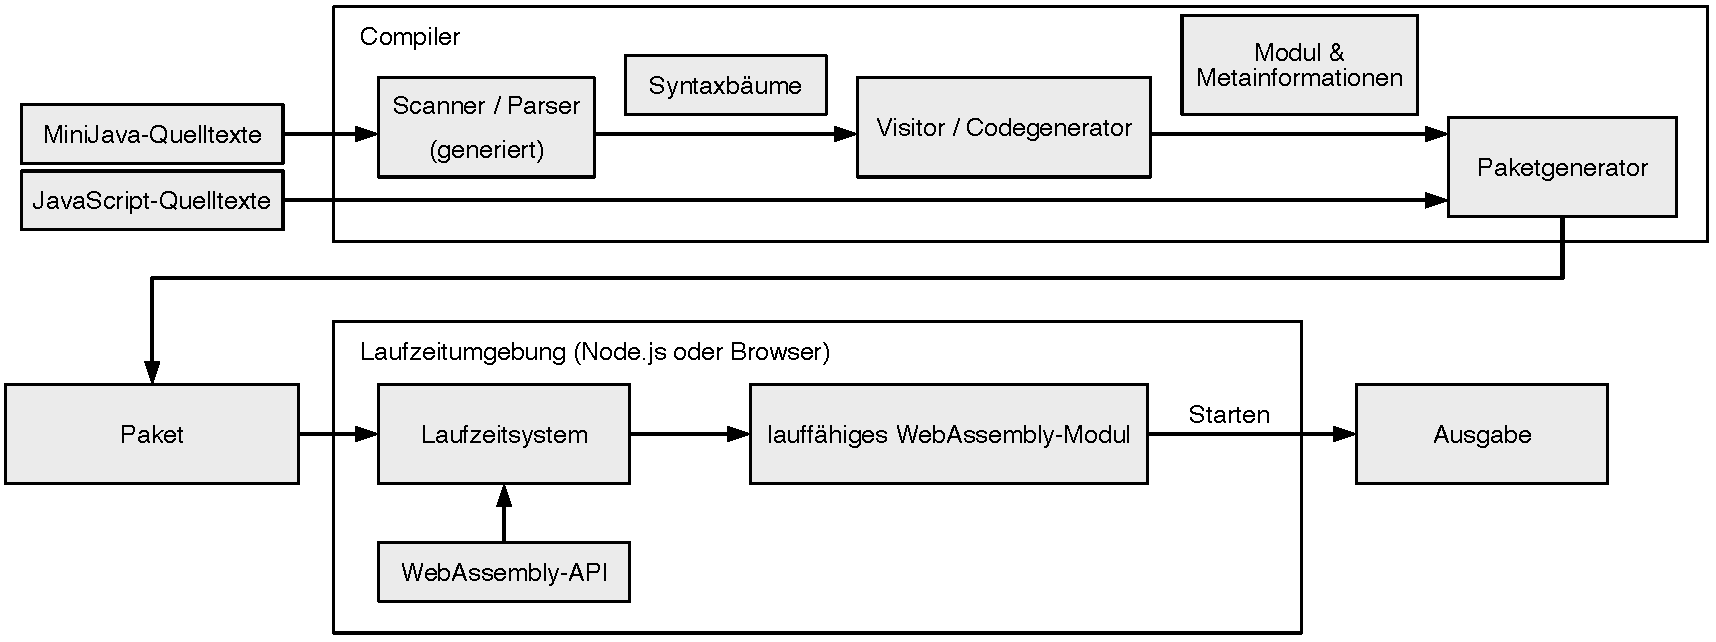
\includegraphics[width=\textwidth]{einleitung/architecture}
    \caption{Architektur des Gesamtsystems}
    \label{fig:architecture}
\end{figure}

\section{Verweis auf Quelltext}
Der Quellcode des gesamten Compilers und der Demo-Beispiele steht auf GitHub zum Download zur Verfügung: \url{https://github.com/stefanschoeberl/TODO}

\chapter{Technische Grundlagen}
\label{cha:Technische-Grundlagen}

In diesem Kapitel werden die technischen Grundlagen beschrieben, auf denen der MiniJava"=Compilers aufgebaut ist. Dazu zählen primär WebAssembly und ANTLR. Weiters wird kurz auf die wichtigsten Hilfstechnologien eingegangen. Außerdem wird anhand ausgewählter Beispiele gezeigt, welche aktuellen Technologien WebAssembly bereits einsetzen oder unterstützen.

\section{WebAssembly}
WebAssembly ist ein Bytecode mit dem Ziel, eine sprachunabhängige Plattform für das Web zu ermöglichen \cite{WebAssemblyWebsite} \cite{WebAssemblySpecification}. So können andere Programmiersprachen (wie zum Beispiel C, C++ oder Rust) und hochperformante Anwendungen in das Web gebracht werden.

\subsection{Hintergrund und Motivation}
Aktuelle Browser unterstützen ausschließlich JavaScript, daher musste bisher der Quelltext anderer Programmiersprachen mit einen Transpiler in JavaScript konvertiert werden. Bei beispielsweise TypeScript übernimmt diese Aufgabe der TypeScript"=Compiler \emph{tsc} \cite{TypeScript}.

JavaScript muss im Browser zur Laufzeit interpretiert werden, gegenbenfalls wird auch ein Just"=In"=Time"=Compiler verwendet \cite{MDNJavaScript}. Dies ist natürlich mit einem gewissen Mehraufwand verbunden. Hier verspricht WebAssembly Performanceverbesserungen, da der Bytecode einfacher geladen (verglichen mit dem Parsen einer Skriptsprache) und effizienter ausgeführt werden kann \cite{WebAssemblySpecification}.

Man könnte auf den ersten Blick vermuten, dass WebAssembly aufgrund des ähnlichen Namen etwas mit \emph{Assembler} gemeinsam hat und man sich daher Gedanken zur Sicherheit machen müsste. Aber deren ist nicht so und WebAssembly gibt ein klares Sicherheitsmodell vor: Vereinfacht beschrieben läuft sämtlicher WebAssembly"=Bytecode im Browser in einer isolierten Umgebung und besitzt nicht mehr Rechte beim Ausführen als JavaScript"=Quelltext \cite{WebAssemblyWebsite} \cite{WebAssemblyW3CPressStandard}.

Im Rahmen eines \emph{Minimum Viable Product} (MVP) entstand die erste Version für WebAssembly, in der nur die notwendigsten Funktionalitäten implementiert wurden, um mit WebAssembly überhaupt arbeiten zu können. \cite{WebAssemblyWebsite}. WebAssembly wird seit 2017 in den vier großen Browsern (Mozilla Firefox, Google Chrome, Apple Safari und Microsoft Edge) unterstützt. Seit Dezember 2019 ist WebAssembly ein offizieller Web"=Standard des W3C (World Wide Web Consortium) \cite{WebAssemblyW3CPressStandard}.

WebAssembly trifft in der Spezifikation keine Annahmen über die Laufzeitumgebung. Auch wenn das derzeit primäre Einsatzgebiet das Web ist, ist es durchaus denkbar, dass WebAssembly auch andersweitig eingesetzt wird. WebAssembly wurde auch so entworfen, dass nicht einmal JavaScript für die Laufzeitumgebung notwendig ist \cite{WebAssemblyWebsite}.

\subsection{Konzepte}
\label{subsec:WebAssembly-Konzepte}
WebAssembly"=Bytecode stellt eine elementare Programmiersprache dar. In der Spezifikation werden für diese einige Konzepte \cite{WebAssemblySpecification} definiert. Nachfolgend werden diese vorgestellt und erklärt.

\begin{description}
    \item[Datentypen] WebAssembly definiert vier Datentypen, zwei für Ganzzahlen und zwei für Fließkommazahlen, jeweils in einer 32"=Bit- und 64"=Bit"=Variante. Der 32"=Bit"=Ganzzahltyp wird auch für Wahrheitswerte und für Speicheradressen verwendet. Die Ganzzahltypen können sowohl für vorzeichenbehafte und vorzeichenlose Zahlen verwendet werden, abhängig von den konkreten Operation darauf werden sie entsprechend interpretiert. Die zwei Ganzzahltypen werden mit \lstinline{i32} und \lstinline{i64} abgekürzt, die zwei Fließkommatypen mit \lstinline{f32} und \lstinline{f64}.
    \item[Instruktionen] Das Laufzeitmodell von WebAssembly basiert auf einer Kellermaschine. Das bedeutet, dass Instruktionen meist Operanden zunächst vom Kellerspeicher herunternehmen, dann die Operation ausführen und am Schluss das Ergebnis wieder auf den Kellerspeicher legen. Standardmäßig werden Instruktionen nacheinander ausgeführt. Es gibt aber auch Instruktionen, die den Kontrollfluss steuern. Einige Instruktionen werden in Abschnitt \ref{subsec:WebAssembly-Instruktionen} detailliert behandelt.
    \item[\emph{Traps}] Instruktionen können (absichtlich oder unbeabsichtigt) Laufzeitfehler in Form von \emph{Traps} erzeugen, die zu einem sofortigen Abbruch der Ausführung führen. Die Behandlung dieser \emph{Traps} erfolgt in der Laufzeitumgebung und nicht direkt in WebAssembly.
    \item[Funktionen] Instruktionen werden in Funktionen gekapselt. Funktionen können beliebig viele Eingangsparameter, maximal ein Funktionsergebnis und beliebig viele lokale Variablen definieren. Funktionen können andere Funktionen oder sich selbst rekursiv aufrufen.
    \item[Tabellen] In Tabellen können derzeit Funktionen abgelegt werden, auf die über einen Index zugegriffen werden kann. Auf diese Art und Weise können beispielsweise Funktionszeiger nachgebildet werden. 
    \item[Linearer Speicher] Linearer Speicher ist ein zusammendhängendes Byte"=Feld, auf das lesend und schreibend zugegriffen werden kann. Der Zugriff erfolgt mit eigenen Instruktionen über einen Index. Beim Erstellen des Speichers wird eine initale Größe definiert, der Speicher kann zur Laufzeit automatisch wachsen.
    \item[Module] In einem Modul werden sämtliche Bestandteile von WebAssembly, darunter Funktionen, Tabellen, Imports und Exports, definiert. Weitere Details zu Modulen finden sich in Abschnitt \ref{subsec:WebAssembly-Module}.
\end{description}

Die Spezifikation fordert nicht, dass Laufzeitumgebungen einen Kellerspeicher zur Auswertung verwalten müssen. Das Programm muss lediglich so ausgeführt werden, als ob es auf einer Kellermaschine laufen würde.

\subsection{Module}
\label{subsec:WebAssembly-Module}
Module sind das Herzstück von WebAssembly. Sämtliche Bestandteile wie beispielsweise Funktionen und deren Implementierung werden als eine Einheit in Form eines Moduls zusammgefasst \cite{WebAssemblySpecification}.

Ein Modul kann textuell oder binär repräsentiert werden. In der Spezifikation werden sämtliche WebAssembly"=Konstrukte in Form einer abstrakten Syntax definiert. Die beiden Darstellungsformen sind somit als Instanzierung dieser abstrakten Syntax zu verstehen. Die abstrakte Syntax definiert eine Baumstruktur. Beide Darstellungeformen sind ineinander umwandelbar. Die binäre Form ist für das \emph{Deployment} vorgesehen, während die textuelle Form als lesbare Darstellung für Menschen gedacht ist \cite{WebAssemblySpecification} \cite{MDNWebAssembly}. Zeilenkommentare sind in der textuellen Darstellung mit \lstinline{;;} möglich.

Die textuelle Darstellung erfolgt in Form von so genannten \emph{S"=Expressions} \cite{WebAssemblySpecification}. Mit diesen können Bäume einfach dargestellt werden. Ein Knoten wird durch \lstinline{(<name> ...)} Ausdrücke beschrieben, zwischen den Klammern befindet sich (durch Leerzeichen getrennt) zuerst der Name/Typ des Knoten, anschließend folgen beliebig viele Werte (zum Beispiel Zahlen oder Zeichenketten) oder Kindknoten \cite{MDNWebAssembly}. In Listing \ref{lst:s-expressions} wird dies anhand eines kleinen Beispiels verdeutlicht.

\lstinputlisting[label={lst:s-expressions}, caption = {Beispiel für \emph{S"=Expressions}: Knoten a hat den Wert 111 und zwei Kindknoten. Diese Kindknoten b und c haben die Werte 222 und 333.}]{src/technischeGrundlagen/sExpressionExample.txt}

Sämtlicher WebAssembly"=Bytecode in dieser Arbeit wird in der textuellen Form mit \emph{S"=Expressions} dargestellt.

In einem Modul können verschiedene Komponenten definiert werden. Nachfolgend wird auf diese im Detail mit Codebeispielen eingegangen.

\begin{description}
    \item[Funktionstypen] Ein Funktionstyp definiert die Schnittstelle einer Funktion. Dabei werden die Datentypen der Eingangsparameter und des Funktionsergebnisses. Auf diese Funktionstypen kann beim Definieren von Funktionen über einen Index zugegriffen werden. Beispielsweise würde der Typ einer Funktion, die zwei 32"=Bit"=Ganzzahlen annimmt und eine 32"=Bit"=Fließkommazahl liefert folgendermaßen definiert werden: \lstinputlisting{src/technischeGrundlagen/modulesType.wat}
    \item[Funktionen] Eine Funktion besteht aus der Signatur und einer Folge von Bytecode"=Instruktionen. Die Signatur kann in der textuellen Darstellung direkt bei der Funktion definiert werden. Alternativ kann ein bestehender Funktionstyp referenziert werden. In einer Funktion können beliebig viele lokale Variablen definiert werden. Angenommen der vorher definierte Funktionstyp wäre über den Index \lstinline{3} erreichbar, könnte man auf folgende zwei Arten eine Funktion mit einer lokalen Variable (64"=Bit Ganzzahl) definieren: \lstinputlisting{src/technischeGrundlagen/modulesFunc.wat}
    Eine Funktion ist über einen Index adressierbar. Dieser Index wird über die Definitionsreihenfolge der Funktionen festgelegt, also erhält die 1. Funktion den Index 0, die 2. Funktion den Index 1 usw.
    \item[Tabellen und Einträge] Diese Funktionsindizes können selbst wieder in Tabellen hinterlegt werden. Damit könnten beispielsweise indirekte Funktionsaufrufe (vergleichbar mit Funktionszeigern) umgesetzt werden. Da für diese Arbeit dieses Konzept nicht relevant ist, wird darauf nicht weiter  eingegangen.
    \item[Linearer Speicher und dessen Initialisierung] Linearer Speicher kann direkt im Modul definiert werden, dabei wird eine Initalgröße (in Anzahl der \emph{Pages}, eine \emph{Page} ist 64KiB groß) angegeben. Der initale Inhalt des Speichers wird über das \lstinline{data}"=Konstrukt definiert. Das folgende Codestück zeigt, wie man beispielsweise einen Speicher definiert (mit Mindestgröße einer Page) und die Zeichenkette \lstinline{"Hello"} an Index 0 ablegt: \lstinputlisting{src/technischeGrundlagen/modulesMemory.wat}
    \item[Globale Variablen] Auf eine globale Variable kann von allen Funktionen aus zugegriffen werden. Eine globale Variabe kann konstant oder veränderbar definiert werden und muss initialisiert werden. Nachfolgend ein Beispiel für zwei 32"=Bit"=Ganzzahlvariablen, einmal konstant und einmal veränderbar. Beide Variablen werden mit \lstinline{123} initialisiert: \lstinputlisting{src/technischeGrundlagen/modulesGlobal.wat}
    \item[Start-Funktion] Jedes Modul kann eine Funktion definieren, die beim Instanzieren des Moduls aufgerufen wird. Die Funktion wird aufgerufen, sobald Tabellen und Speicher initialisiert wurden. Die aufzurufende Funktion wird über den Index angegeben. Nachfolgend sieht man, wie beispielsweise die Funktion mit Index \lstinline{12} als Startfunktion definiert wird: \lstinputlisting{src/technischeGrundlagen/modulesStart.wat}
    \item[Importe] Funktionen, Tabellen, Speicher und globale Variablen können von der Laufzeitumgebung zur Verfügung gestellt werden. Ein Import besteht aus drei Teilen: aus einem Modulnamen, Objektnamen und Objektdefinition. Der Modulname ist nicht mit einem WebAssembly- oder JavaScript"=Modul gleichzusetzen, Modulname und Objektname bilden gemeinsam einen zweistufigen Bezeichner, der flexibel nach Bedarf verwendet werden kann. So würde man beispielsweise die Funktion \lstinline{env.println} importieren, der Funktionstyp wäre hier mit Index \lstinline{1} definiert: \lstinputlisting{src/technischeGrundlagen/modulesImport.wat}
    Über Importe kann in WebAssembly direkt nach außen kommuniziert werden. Auf diese Art können beispielsweise Konsolenausgaben umgesetzt werden.
    \item[Exporte] Funktionen, Tabellen, Speicher und globale Variablen können auch der Laufzeitumgebung zugänglich gemacht werden. Die Definition eines Exports ist etwas einfacher als die eines Imports, da hier kein Modulname notwendig ist. So würde man beispielsweise die Funktion mit Index 3 als \lstinline{main} exportieren: \lstinputlisting{src/technischeGrundlagen/modulesExport.wat}
    Mit Exporte kann die Umgebung mit dem WebAssembly"=Modul kommunizieren. Die Umgebung kann dadurch beispielsweise Funktionen im Modul aufrufen.
\end{description}

\subsection{Instruktionen}
\label{subsec:WebAssembly-Instruktionen}
WebAssembly unterstützt eine Reihe von elementaren Bytecode"=Instruktionen. Instruktionen können zur Compilezeit festgelegte Argumente annehmen. Nachfolgend wird auf einige ausgewählte Instruktionen im Detail eingegangen. Eine vollständige Liste aller Instruktionen findet sich in der WebAssembly"=Spezifikation \cite{WebAssemblySpecification}. (Anmerkung: Die meisten Instruktionen existieren in Ausprägungen für jeden der vier elementaren Datentypen. Die nachfolgenden Beispiele werden nur anhand des 32"=Bit"=Ganzzahltyps gezeigt, \lstinline{i32} könnte man somit mit einem anderen Datentyp ersetzen.)

Die Instruktion \lstinline{i32.const} legt zur Laufzeit eine zur Compilezeit definierte Konstante auf den Kellerspeicher, zum Beispiel: \lstinline{i32.const 123}.

Lokale Variablen lassen sich mit \lstinline{local.get} und \lstinline{local.set} lesen und schreiben. Die lokalen Variablen werden ab \lstinline{0} beginnend nummeriert. Hat eine Funktion Parameter, so zählen die Parameter ebenfalls zu den lokalen Variablen. Der erste Parameter bekommt die Nummer \lstinline{0}, danach folgen die lokalen Variablen.

\lstinline{local.get} liest den Wert der angeforderten lokalen Variable und legt den Wert auf den Kellerspeicher. \lstinline{local.set} holt einen Wert vom Kellerspeicher und speichert diesen in die angegebene Variable. In Listing \ref{lst:wasm-locals} wird das Lesen der ersten lokalen Variable und das Schreiben ihres Werts in die zweite lokale Variable dargestellt, dies entspricht einer einfachen Zuweisung wie \lstinline{a = b}. 

\lstinputlisting[label={lst:wasm-locals}, caption={Lesen und Schreiben lokaler Variablen}]{src/technischeGrundlagen/instructionsLocal.wat}

Für das Rechnen mit Variablen bietet WebAssembly eine Reihe an binären Operationen an. Diese nehmen jeweils die obersten zwei Werte vom Kellerspeicher herunter (Operanden), wenden auf diese die Operation an und legen anschließend das Ergebnis oben auf den Kellerspeicher. Hier drei Beispiele für solche Instruktionen: \lstinline{i32.add} (Addieren), \lstinline{i64.and} (Bitweises Und), \lstinline{f32.le} (Kleiner oder gleich, \emph{lower or equal}).

Weiters gibt es einige strukturierte Instruktionen zur Steuerung des Kontrollflusses. Die einfachste ist die binäre Verzweigung, sie besteht aus drei Instruktionen: \lstinline{if}, \lstinline{else} und \lstinline{end}. Die \lstinline{if}"=Instruktion nimmt einen Wert vom Kellerspeicher. Ist dieser ungleich 0, also \emph{wahr}, werden die Instruktionen zwischen \lstinline{if} und \lstinline{else} ausgeführt. Ist der Wert am Kellerspeicher gleich 0, \emph{falsch}, werden die Instruktionen zwischen \lstinline{else} und \lstinline{end} ausgeführt. In Listing \ref{lst:wasm-if-else-end} ist ein Beispiel dargestellt.

\lstinputlisting[label={lst:wasm-if-else-end},caption = {Beispiel einer binären Verzweigung: Abhängig vom Wert in der ersten lokalen Variable wird \lstinline{1} oder \lstinline{2} in die zweite lokale Variable geschrieben. Rechts daneben ist als Kommentar dazu äquivalenter Pseudocode dargestellt.}]{src/technischeGrundlagen/instructionsIfElseEnd.wat}

Zusätzlich zu der binären Verzweigung sind auch Sprünge möglich. Es ist allerdings nicht möglich, zu jeder beliebigen Instruktion im Bytecode zu springen. Sprungziele werden mit \lstinline{block ... end} oder \lstinline{loop ... end} definiert. Dabei wird beim Betreten des Bereichs ein Sprungziel auf den Kellerspeicher gelegt. Beim Verlassen des Bereichs wird das Sprungziel wieder vom Kellerspeicher genommen. Somit sind die Sprungziele nur innerhalb des Bereichs gültig. Das Sprungziel ist bei \lstinline{block} das Ende des Bereichs, bei \lstinline{loop} der Anfang des Bereichs. Einen (unbedingten) Sprung kann man mit der \lstinline{br}"=Instruktion durchführen. Für einen bedingten Sprung ist die \lstinline{br_if}"=Instruktion vorgesehen, dabei wird ein Wert zunächst vom Kellerspeicher genommen. Nur wenn dieser wahr (ungleich 0) ist, wird gesprungen. Beide Sprunginstruktionen erwarten als Argument eine Zahl \lstinline{n}. Die Instruktion führ dann einen Sprung zum \lstinline{n}"=ten Sprungziel am Kellerspeicher durch. Diese Instruktionen können für Schleifen eingesetzt werden. In Listing \ref{lst:wasm-loop} ist ein Beispiel dargestellt.

\lstinputlisting[label={lst:wasm-loop}, caption = {Beispiel für eine einfache Schleife: Am Anfang der Schleife wird der Wert der ersten lokalen Variable ausgelesen. Ist dieser wahr, wird die Schleife verlassen. Am Ende der Schleife wird unbedingt zum Anfang der Schleife gesprungen. Rechts daneben ist als Kommentar dazu äquivalenter Pseudocode dargestellt.}]{src/technischeGrundlagen/instructionsBranches.wat}

Funktionen können mit der \lstinline{call}"=Instruktion aufgerufen werden. Die Instruktion benötigt als Argument den Index der aufzurufenden Funktion, zum Beispiel: \lstinline{call 1}. Falls die aufgerufene Funktion einen Rückgabewert liefert, liegt dieser nach dem Funktionsaufruf auf dem Kellerspeicher. Daher muss in der Implementierung einer Funktion mit Rückgabewert dieser am Ende der Funktion auf den Kellerspeicher gelegt werden.

Eine Funktion kann frühzeitig mit der \lstinline{return}"=Instruktion verlassen werden. Liefert die Funktion einen Rückgabewert, muss dieser vor der \lstinline{return}"=Instruktion auf den Kellerspeicher gelegt werden.

Ein Laufzeitfehler kann bewusst mit der \lstinline{unreachable}"=Instruktion ausgelöst werden. Diese Instruktion löst immer eine \emph{Trap} aus.

\subsection{Aktueller Entwicklungsstand und zukünftige Entwicklungen}
Wie bereits beschrieben wurde im MVP von WebAssembly nur die allernotwendigste Funktionalität spezifiziert und implementiert. Neue Funktionalitäten durchlaufen einen Standardisierungsprozess \cite{WebAssemblyW3CProcess}. Dieser besteht aus sechs Phasen, die Phasen werden mit 0 beginnend nummeriert:

\begin{enumerate}
    \setcounter{enumi}{-1}
    \item \emph{Pre-Proposal}: Ein Mitglied der \emph{Community Group} hat eine Idee und erstellt eine quasi"=formale Beschreibung. Die \emph{Community Group} stimmt für oder gegen Idee.
    \item \emph{Feature Proposal}: Die Funktionalität wird in einem offiziellen \emph{Repository} aktiv entworfen. Wenn notwendig können Prototypen implementiert werden.
    \item \emph{Proposed Spec Text Available}: Eine vollständige Spezifikation in Englisch ist nun vorhanden. In dieser Phase wird an mindestens einer Implementierung entwickelt, sodass Tests mit dieser ausgeführt werden können. Diese Tests werden in einer Testsuite zusammengefasst.
    \item \emph{Implementation Phase}: Die Testsuite ist nun vollständig und mindestens eine Implementierung durchläuft diese fehlerfrei. Nun müssen sogenannte \emph{Embedder} die Funktionalität implementieren. Die Spezifikation wird weiter verfeinert. Die Referenzimplementierung und Werkzeuge werden um die neue Funktionalität ergänzt.
    \item \emph{Standardize the Feature}: Nun sind einige Implementierungen vollständig und die Spezifikation ist eingefroren, nur noch kleine kosmetische Anpassungen werden vorgenommen. Ab jetzt übernimmt die \emph{Working Group}. Regelmäßig wird über die Nützlichkeit der Funktionalität abgestimmt.
    \item \emph{The Feature is Standardized}: Die Funktionalität ist fertiggestellt und wurde in die Spezifikation aufgenommen.
\end{enumerate}

Sämtliche aktive Entwicklungen werden in einem GitHub"=\emph{Repository} zusammengefasst \cite{WebAssemblyProposals}.
Einige davon haben bereits die Implementierungsphase (4) erreicht, beispielsweise Unterstützung für Referenzdatentypen. \emph{Threads} befinden sich beispielsweise erst in Phase 2. Interessante Funktionalitäten wie \emph{Garbage Collection} oder \emph{Interface Types} (diese sollen dabei helfen, die Interoperabilität mit Web"=APIs zu verbessern \cite{WebAssemblyInterfaceTypes}) sind erst in Phase 1.

\subsection{\emph{WebAssembly Binary Toolkit}}
Das \emph{WebAssembly Binary Toolkit} (WABT) ist eine Sammlung an Werkzeugen, die EntwicklerInnen im Kontext von WebAssembly unterstützen sollen \cite{WABT}. Dazu zählen Werkzeuge zum Analysieren, Validieren und Dekompilieren von WebAssembly"=Modulen. Zwei im Rahmen dieser Arbeit nützliche Werkzeuge sind \lstinline{wat2wasm} und \lstinline{wasm2wat}, mit denen zwischen der textuellen und binären Repräsentation eines Moduls hin und her konvertiert werden kann. Konkret wird \lstinline{wat2wasm} im MiniJava"=Compiler eingesetzt, um das binäre WebAssembly"=Modul zu generieren.

\subsection{JavaScript-API}
\label{subsec:WebAssembly-JavaScript-API}
JavaScript stellt eine Schnittstelle zur Verfügung, mit der WebAssembly"=Module geladen, kompiliert und ausgeführt werden können \cite{MDNWebAssembly}. In diesem Abschnitt soll ein Überblick über diese Schnittstelle gegeben werden.

Zunächst muss das Modul geladen werden. Dies kann im Browser beispielsweise mit \lstinline{fetch} und in Node.js mit \lstinline{fs.readFile} erfolgen. Mit \lstinline{WebAssembly.compile} wird aus diesen Rohdaten das Modul kompiliert. Im Browser können diese zwei Schritte auch gemeinsam mit \lstinline{WebAssembly.compileStreaming} zusammengefasst werden, dabei wird während des Herunterladens das Modul gleichzeitig kompiliert. Dadurch können schnellere Ladezeiten erreicht werden. Diese Funktion ist allerdings nicht in allen Browsern verfügbar.

Nun wird mit \lstinline{WebAssembly.instantiate} eine Instanz des Moduls erzeugt. Diese Funktion benötigt als weiteren Parameter ein JavaScript"=Objekt, das die Imports definiert. In diesem Import"=Objekt spiegelt sich der zweistufige Bezeichner wieder. So könnte man beispielsweise die in Abschnitt \ref{subsec:WebAssembly-Module} importierte Funktion \lstinline{env.println} bereitstellen:

\lstinputlisting{src/technischeGrundlagen/importObject.js}

Die Schritte Herunterladen, Kompilieren und Instanzieren lassen sich ebenfalls mit der (nicht in allen Browsern unterstützten) Funktion \lstinline{WebAssembly.instantiateStreaming} zusammenfassen.

Man erhält am Ende die Modulinstanz als JavaScript"=Objekt. Dieses Objekt hat die Datenkomponente \lstinline{exports}. Über diese können exportiere Funktionen aufgerufen werden.

In Listing \ref{lst:wasm-js-api} findet sich ein zusammenhängendes Beispiel, um das Zusammenspiel zwischen WebAssembly und JavaScript zu veranschaulichen.

\lstinputlisting[label={lst:wasm-js-api}, caption = {Beispiel aus der MDN"=Dokumentation \cite{MDNWebAssembly}: In JavaScript wird die exportierte Funktion \lstinline{exported_func} aufgerufen, diese ruft wiederum \lstinline{imported_func} auf. Das Programm gibt zur Laufzeit \lstinline{42} auf der Konsole aus.}]{src/technischeGrundlagen/simpleJSAPI.txt}

\section{ANTLR}

ANTLR (ANother Tool for Language Recognition) ist ein von Terence Parr entwickelter Scanner- und Parsergenerator, der Quelltext für diverse Programmiersprachen (darunter Java und C\#{}) generiert \cite{ANTLR4Reference} \cite{ANTLRWebsite}. ANTLR selbst ist in Java geschrieben. Die Programmiersprache, für die Scanner und Parser generiert werden, wird nachfolgend auch als Zielsprache bezeichnet. Unter \emph{ANTLR} ist in der gesamten Arbeit die aktuelle Hauptversion 4 zu verstehen, außer es wird explizit anders angegeben.

\subsection{Parser}

ANTLR ist in der Lage, für jede kontextfreie Grammatik ohne indirekte oder versteckte Linksrekursion einen Parser zu erzeugen \cite{ANTLRALLStar}. Eine indirekte Linksrekursion ist beispielsweise in folgenden Regeln enthalten: $A \rightarrow B.\ B \rightarrow A.$ \cite{ANTLRALLStar}. Eine versteckte Linksrekursion findet sich beispielsweise in diesen Regeln: $A \rightarrow B A.\ B \rightarrow \epsilon.$ \cite{ANTLRALLStar}. Der Parser arbeitet nach dem Prinzip des rekursiven Abstiegs. Das dabei eingesetzt Verfahren heißt ALL(*) (Adaptive LL(*)). In diesem Abschnitt wird das Verfahren nur überblicksmäßig erläutert, weitere Details dazu sind in \cite{ANTLR4Reference}, \cite{ANTLRLLStar} und \cite{ANTLRALLStar} nachzulesen.

ALL(*) basiert auf dem in ANTLR 3 eingesetzten LL(*). LL(*) unterscheidet sich von LL(k) dahingehend, dass die Anzahl der Vorgriffssymbole nicht fixiert ist \cite{ANTLRLLStar}. Beim Treffen einer Entscheidung bei Alternativen wird stattdessen ein regulärer Ausdruck verwendet. ANTLR 3 erzeugt beim Generieren des Parsers für jedes Nonterminalsymbol einen deterministischen endlichen Automat. Gelingt es nicht, einen solchen Automanten zu erzeugen, wird auf \emph{Backtracking} zurückgegriffen.

ALL(*) erweitert die Idee von LL(*): Hier wird der determinische endliche Automat beim Parsen dynamisch erzeugt \cite{ANTLRALLStar}. Beim Erzeugen des Automaten werden die Symbole der tatsächlichen Eingabe verwendet. Beim Treffen zukünftiger Entscheidungen wird der bestehende Automat verwendet oder wenn notwendig erweitert. Der Vorteil gegenüber LL(*) ist, dass beim Aufbau des deterministischen endlichen Automaten zur Laufzeit nur eine endliche Menge an Eingaben berücksichtigt werden muss, während bei LL(*) \emph{alle} Möglichkeiten von potenziellen Eingaben berücksichtigt werden müssen.

ALL(*) kann mit kontextfreien Grammatik ohne indirekte oder versteckte Linksrekursion umgehen \cite{ANTLR4Reference} \cite{ANTLRALLStar}. ANTLR ist jedoch in der Lage, direkte Linksrekursionen aufzulösen. Dadurch lassen sich mathematische Ausdrücke übersichtlicher und kompakter schreiben. Der Vorrang der Operatoren wird durch die Reihenfolge der Alternativen beschrieben: Die Priorität nimmt von oben nach unten ab. Bei den Operatoren wird standardmäßig Linksassoziativität angenommen, benötigt man Rechtsassoziativität, muss dies explizit angegeben werden. So kann aus einer eigentlich mehrdeutigen Grammatik ein eindeutiger Syntaxbaum aufgebaut werden. In Listing \ref{lst:antlr-left-recursion} findet sich ein Beispiel um das zu verdeutlichen.

\pagebreak
\lstinputlisting[label={lst:antlr-left-recursion}, caption = {Beispiel für mathematische Ausdrücke in ANTLR \cite{ANTLR4Reference}}]{src/technischeGrundlagen/antlrMathExpressions.g4}

Insgesamt lassen sich durch das automatische Auflösen von Linksrekursionen und durch ALL(*)"=Grammatiken schreiben, die nicht zu stark auf das darunterliegende Parser"=Verfahren angepasst werden müssen \cite{ANTLR4Reference}. Ein extremes Gegenbeispiel dazu ist die (händische) Transformation einer Grammatik, sodass die daraus entstehende Grammatik LL(1)"=konform ist.

\subsection{Grammatikbeschreibung}

Die Grammatik einer Sprache wird in einer Textdatei mit dem Dateityp \lstinline{g4} beschrieben. In Listing \ref{lst:antlr-listOfNumbers-grammar} ist ein einfaches Beispiel für eine Grammatik, die benannte Zahlenlisten beschreibt, zum Beispiel \lstinline{even[ 2 4 ]}, \lstinline{empty[ ]} oder \lstinline{prime[ 2 3 5 7 ]}. In Abbildung \ref{fig:syntaxtree} wird der Syntaxbaum des Satzes \lstinline{even[ 2 4 ]} dargestellt.

\lstinputlisting[label = {lst:antlr-listOfNumbers-grammar}, caption = {\emph{MyLanguage.g4}}]{src/technischeGrundlagen/MyLanguage.g4}

\begin{figure}[b]
    \centering
    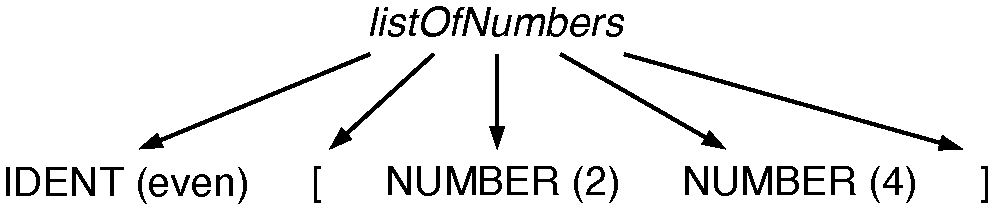
\includegraphics[width=0.6\textwidth]{technischeGrundlagen/syntaxtree}
    \caption{Syntaxbaum des Satzes \lstinline{even[ 2 4 ]}}
    \label{fig:syntaxtree}
\end{figure}

Am Beginn steht der Name der Grammatik. Anschließend folgen Regeln für Nonterminalsymbole und zum Schluss Terminalsymbole. Formatierungen wie Leerzeichen, Zeilenumbrüche usw. können ignoriert werden. Dafür ist das Terminalsymbol \lstinline{WS} (steht für \emph{white space}) zuständig. Mit \lstinline{-> skip} werden in diesem Fall Leerzeichen, Tabulatorzeichen und Zelenendezeichen ignoriert, sodass man sich in der Grammatik darum nicht mehr kümmern muss. Das \lstinline{*}"=Symbol kennzeichnet $0$ bis $n$ Wiederholungen des vorherigen Ausdrucks, das \lstinline{+}"=Symbol kennzeichnet $1$ bis $n$ Wiederholungen.

Beim Parsen entsteht aus einem Eingabetext ein Syntaxbaum. Nonterminalsymbole stellen Knoten in diesem Baum dar, Terminalsymbole sind darin Blattknoten. Kindknoten lassen sich in diesem Syntaxbaum auch benennen. Zu einem \lstinline{listOfNumbers}"=Knoten aus dem obigen Beispiel wird das Terminalsymbol \lstinline{IDENT} mit \lstinline{name} benannt. Der Knoten im Syntaxbaum erhält dann eine Datenkomponente \lstinline{name}, die auf das Terminalsymbol verweist. Es können auch mehrere Kindknoten in einer Liste gespeichert werden (dies erfolgt mit dem Operator \lstinline{+=}), in diesem Fall werden alle \lstinline{NUMBER}-Terminalsymbole in der Datenkomponente \lstinline{numbers} zusammengefasst.

Aus der Grammatikdatei werden Scanner, Parser und weitere Hilfsklassen mit dem ANTLR"=Werkzeug\footnote{\url{https://www.antlr.org/download/antlr-4.8-complete.jar}} erzeugt. Dieser Prozess lässt sich außerdem in Gradle über ein Plugin integrieren \cite{GradleANTLRPlugin}.

\subsection{Integration in Kotlin}

Aus der im vorherigen Abschnitt beschriebenen Grammatik kann mit ANTLR nun Quelltext für die Zielsprache Java erzeugt werden. Die Namen der generierten Dateien beginnen mit dem Grammatiknamen. Der erzeugte Scanner und Parser wird nun in ein eigenes Programm integriert.

Da sich Java von Kotlin aus verwenden lässt, findet sich in Listing \ref{lst:antlr-kotlin-usage} ein Beispiel, wie der generierte Scanner und Parser in Kotlin aufgerufen wird. 

\lstinputlisting[label = {lst:antlr-kotlin-usage}, caption = {Verwendung der generierten ANTLR"=Klassen in Kotlin}]{src/technischeGrundlagen/antlrKotlin.kt}

Zu den einzelnen Zeilen ein paar Details:
\begin{itemize}
    \item In Zeile 1 wird aus dem Inhalt der Datei mit dem Namen \lstinline{"..."} ein Strom an Zeichen erzeugt.
    \item In Zeile 2 wird aus der generierten Klasse \lstinline{MyLanguageLexer} und dem Zeichenstrom ein \lstinline{Lexer}"=Objekt erzeugt.
    \item In Zeile 3 wird aus dem \lstinline{Lexer}"=Objekt ein Strom an Terminalsymbolen (\lstinline{Tokens}) erzeugt.
    \item In Zeile 4 wird aus der generierten Klasse \lstinline{MyLanguageParser} und dem Strom an Terminalsymbolen ein \lstinline{Parser}"=Objekt erzeugt.
    \item In Zeile 5 wird ein Syntaxbaum beginnend mit dem Satzsymbol \lstinline{listOfNumbers} aufgebaut.
\end{itemize}

\pagebreak
\subsection{Semantische Aktionen}

Oft reicht es nicht, lediglich zu überprüfen, ob ein Text in der Sprache der Grammatik enthalten ist. Besonders beim Parsen von Programmiersprachen müssen anhand des konkreten Quelltextes Entscheidungen oder semantische Aktionen getroffen werden. ANTLR bietet hier zwei Ansätze an:

\begin{itemize}
    \item Die Struktur der Sprache wird in einer Grammatik beschrieben. Semantische Aktionen stehen davon getrennt in eigenen Komponenten (\lstinline{Listener} oder \lstinline{Visitor}), die den Syntaxbaum auswerten. Die Grammatik enthält keinen zielsprachenspezifischen Quelltext.
    \item Die Grammatik enthält zielsprachenspezifischen Quelltext in Form von Codeeinschlüssen. Diese Einschlüsse werden im generierten Scanner bzw. Parser eingebettet und später während dem Scannen und Parsen ausgeführt. 
\end{itemize}

Parr empfiehlt, soweit als möglich auf Codeeinschlüsse zu verzichten. Dafür sprechen folgende Argumente \cite{ANTLR4Reference}:
\begin{itemize}
    \item Saubere Trennung von Grammatik und Auswertung im Sinne des \emph{Single-res\-pon\-si\-bi\-li\-ty principle} \cite{AgileSoftwareDevelopmentPPP}.
    \item Da die Grammatik zielsprachunabhängig bleibt, können Scanner und Parser einfacher für andere Zielsprachen aus bestehenden Grammatiken erzeugt werden.
    \item Die Grammatik bleibt übersichtlicher, da Quelltext der Zielsprache nicht mit Grammatikregeln verwoben ist.
\end{itemize}

Dennoch kann es Gründe geben, die für Codeeinschlüsse sprechen:
\begin{itemize}
    \item Wenn nur wenige semantische Aktionen benötigt werden und der Quelltext der gesamten Anwendung so übersichtlicher bleibt.
    \item Um sich das Aufbauen des Syntaxbaums im Arbeitsspeicher zu ersparen. Dies ist zum Beispiel bei performancekritischen Anwendungen wichtig.
    \item Manchmal ist es notwendig, Entscheidungen im Parsevorgang selbst treffen zu müssen (zum Beispiel für \emph{Predicated parsing}).
    \item Die Generierung für mehrere Zielsprachen ist nicht notwendig.
    \item Die Wiederverwendbarkeit der Grammatik steht nicht im Vordergrund.
\end{itemize}

\begin{figure}[b]
    \centering
    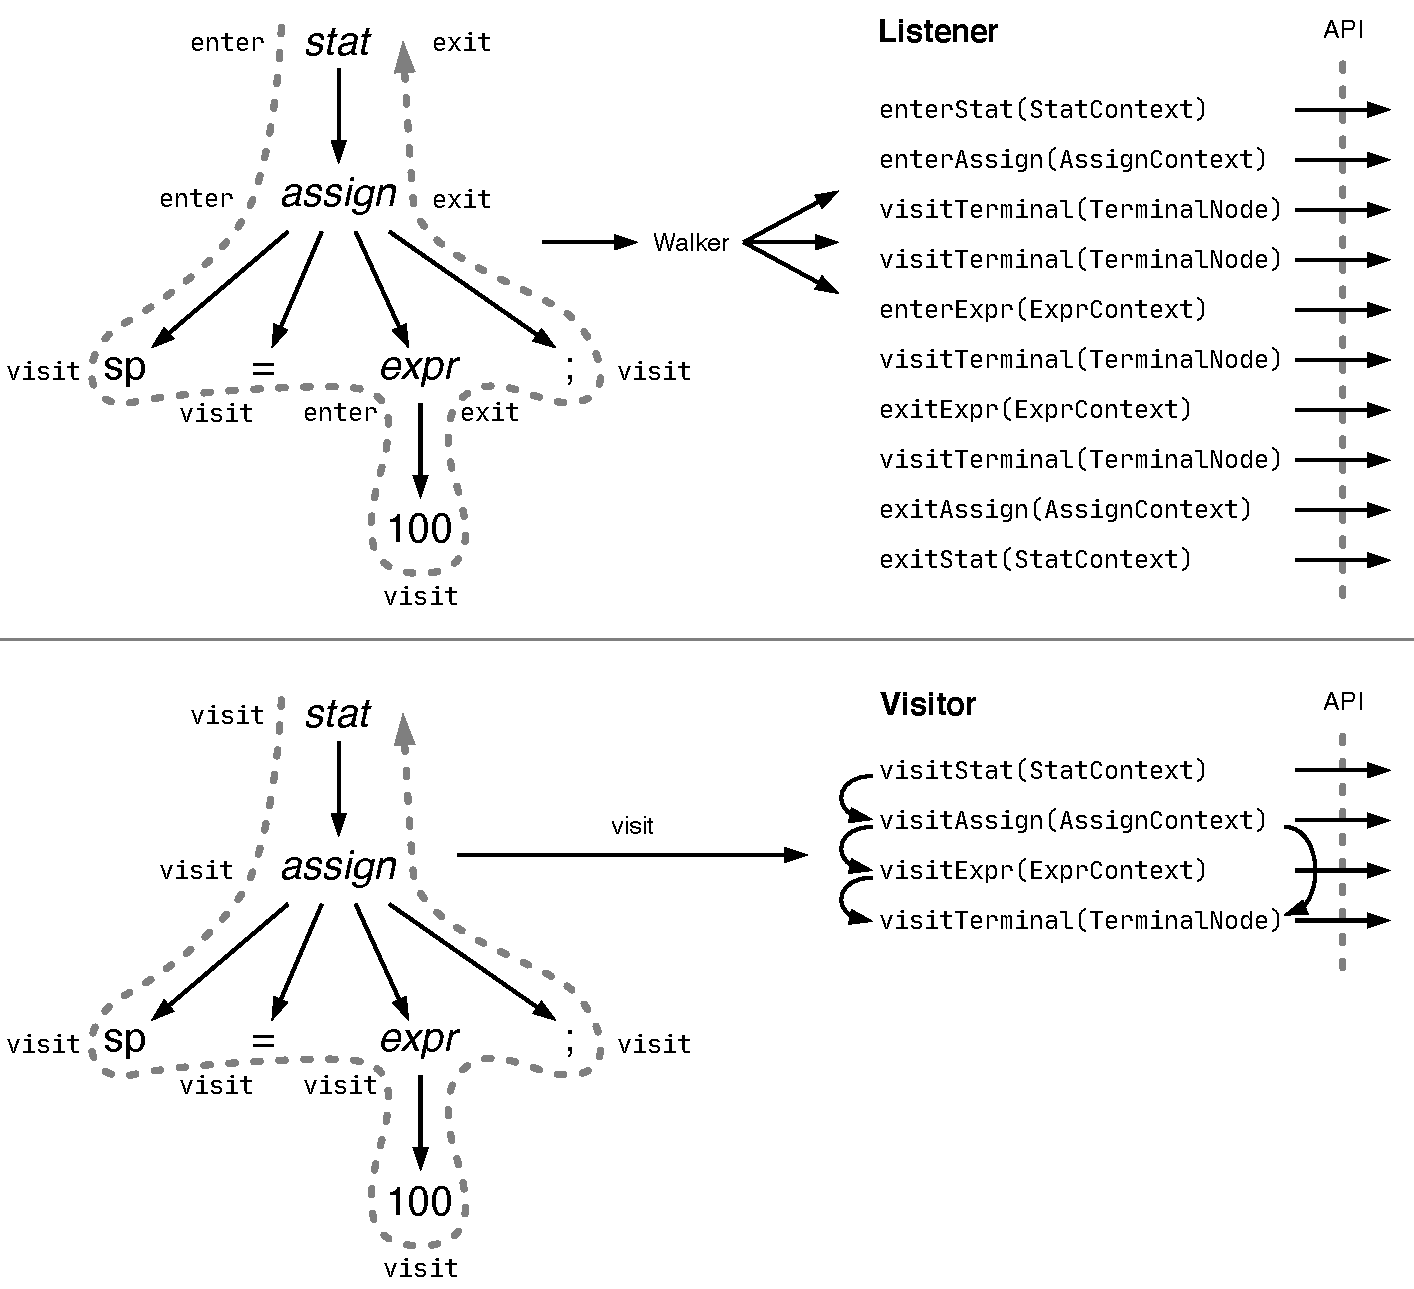
\includegraphics[width=\textwidth]{technischeGrundlagen/listenerVisitor}
    \caption{Abarbeiten des Syntaxbaums des Satzes \lstinline{x = 100;} mit einem \lstinline{Listener} und \lstinline{Visitor} \cite{ANTLR4Reference}}
    \label{fig:listenerVisitor}
\end{figure}

In dieser Arbeit wurde der Ansatz mit sauberer Trennung von Grammatik und Auswertung umgesetzt. Wie bereits erwähnt, bietet ANTLR dafür mit \lstinline{Listener} und \lstinline{Vistor} zwei Möglichkeiten, um den Syntaxbaum auszuwerten. In Abbildung \ref{fig:listenerVisitor} werden die beiden Ansätze visuell gegenübergestellt. Nachfolgend werden die zwei Ansätze im Detail beschrieben.

Die einfachste Art, einen Syntaxbaum abzuarbeiten besteht aus einer Kombination aus einem \lstinline{ParseTreeWalker} und einem \lstinline{Listener}. Das Prinzip ist hier vergleichbar mit dem Verarbeiten von XML"=Dokumenten auf Basis von SAX. ANTLR stellt den \lstinline{ParseTreeWalker} zur Verfügung, der \lstinline{Listener} ist auf Basis eines generierten \emph{Interfaces} selbst zu implementieren. Der Syntaxbaum wird vom \lstinline{ParseTreeWalker} in einer \emph{depth"=first}"=Reihenfolge abgearbeitet. Beim Betreten und Verlassen eines Knoten werden bei Nonterminalsymbolen entsprechende \lstinline{enter}- und \lstinline{exit}"=Methoden des \lstinline{Listeners} aufgerufen, bei Terminalsymbolen gibt es nur die Methode \lstinline{visitTerminal}.

Manchmal ist jedoch etwas mehr Kontrolle notwendig: Zum Beispiel wenn man den Baum in einer anderen Reihenfolge auswerten möchte. Es kann auch sein, dass Teile des Syntaxbaums gar nicht ausgewertet werden müssen. Hier muss basierend auf einem generierten \emph{Interface} ein \lstinline{Visitor} implementiert werden. Für jeden Knotentyp gibt es eine Methode nach dem Schema \lstinline{visitXYZ}. In der Implementierung der \lstinline{visit}"=Methoden muss, sofern erwünscht, aktiv das Abarbeiten von Kindknoten angestoßen werden.

ANTLR generiert zu jedem \lstinline{Listener}- und \lstinline{Visitor}"=\emph{Interface} eine Basisimplementierung, in der beim \lstinline{Listener} alle Methoden leer sind und beim \lstinline{Visitor} alle Kinder abgearbeitet werden. So müssen in eigenen Implementierung nur die relevanten Methoden überschrieben werden.

\pagebreak
\section{Weitere Technologien}

Neben WebAssembly und ANTLR als Kerntechnologien werden für die Implementierung einige Hilfstechnologien benötigt. Auf diese wird in diesem Abschnitt eingegangen.
\subsection{Kotlin}
Kotlin ist eine von JetBrains entwickelte Programmiersprache \cite{KotlinReference}. Kotlin zeichnet sich besonders durch die kompakte Syntax und starke Integration in das bestehende Java"=Umfeld aus. Zusätzlich bietet Kotlin Absicherungen gegen \lstinline{NullPointerExceptions} zur Übersetzungszeit. Wie bei Java wird aus Kotlin beim Kompilieren Bytecode für die \emph{Java Virtual Machine} (JVM) erzeugt. Durch diese enge Interoperabilität kann beim Programmieren mit Kotlin auf die bereits große Menge an Java"=Bibliotheken zurückgegriffen werden.

Die kompakte Syntax von Kotlin gegenüber Java wird anhand eines kleinen Beispiels mit \emph{Data Classes} gezeigt. Mit \emph{Data Classes} können Klassen, die primär nur Daten kapseln, sehr einfach definiert werden, da oft benötigte Methoden wie \emph{Getter}, \emph{Setter}, \lstinline{hashCode}, \lstinline{equals} und \lstinline{toString} automatisch vom Kotlin"=Compiler erzeugt werden. Außerdem wird ein Konstruktor generiert, mit dem alle Datenkomponenten initialisiert werden können. In Java müsste man all diese Methoden händisch schreiben oder von der IDE generieren lassen. In Listings \ref{lst:point-kotlin} und \ref{lst:point-java} wird der Quelltext für die Klasse \lstinline{Point} gezeigt. Die Unterschiede sind deutlich sichtbar.

\lstinputlisting[label = {lst:point-kotlin}, caption = {Die Klasse \lstinline{Point} in Kotlin}]{src/technischeGrundlagen/Point.kt}

\lstinputlisting[label = {lst:point-java}, caption = {Die Klasse \lstinline{Point} in Java. Konstruktor, \emph{Getter}, \emph{Setter}, \lstinline{hashCode}, \lstinline{equals} und \lstinline{toString} wurden von IntelliJ generiert.}]{src/technischeGrundlagen/Point.java}

Kotlin bietet wie bereits erwähnt Absicherungen gegen \lstinline{NullPointerExceptions} zur Übersetzungszeit. Ein einfaches Beispiel dafür findet sich in Listing \ref{lst:npe-kotlin}.

\lstinputlisting[label = {lst:npe-kotlin}, caption = {Beispiel für die Absicherungen gegen \lstinline{NullPointerExceptions}. Die Methode \lstinline{findPoint} liefert als Rückgabewert die Referenz auf ein \lstinline{Point}"=Objekt oder \lstinline{null}, dies wird durch das Fragezeichen gekennzeichnet. Da die lokale Variable \lstinline{point} in Zeile 5 nach dem Aufruf \lstinline{null} sein kann und ein Zugriff auf die \lstinline{x}"=Datenkomponente zu einer \lstinline{NullPointerException} führen könnte, wird ein Übersetzungsfehler ausgelöst. Nach der Prüfung in Zeile 6 kann garantiert werden, dass \lstinline{point} nicht \lstinline{null} ist, somit kann in Zeile 7 gefahrlos auf die Datenkomponente zugegriffen werden.}]{src/technischeGrundlagen/nullSaftety.kt}

Bei MiniJava wird Kotlin als Implementierungssprache des MiniJava"=Compilers eingesetzt. Der von ANTLR generierte Parser (Java"=Quelltext) lässt sich von Kotlin ausgehend problemlos verwenden. Kotlin wurde aufgrund persönlicher Präferenz gewählt, da die tatsächliche Implementierungssprache des Compilers im JVM"=Umfeld keine essenzielle Rolle spielt.

\pagebreak
\subsection{Node.js}
Node.js ist eine JavaScript"=Laufzeitumgebung, die auf der V8"=JavaScript"=Engine aufbaut \cite{NodeJSDocumentation}. Node.js wird unter anderem bei skalierbaren Serveranwendungen eingesetzt, die möglichst viele Verbindungen gleichzeitig abarbeiten können sollen. Node.js unterstützt die JavaScript"=API für WebAssembly (siehe Abschnitt \ref{subsec:WebAssembly-JavaScript-API}).

Bei MiniJava wird Node.js als Laufzeitumgebung für Konsolenanwendungen eingesetzt.

\subsection{JavaScript}
JavaScript ist eine Skriptsprache, die zur Laufzeit interpretiert wird \cite{MDNJavaScript}. Bekannt ist sie vor allem als clientseitige Programmiersprache im Browser für Webseiten. JavaScript ist prototypbasiert und dynamisch typisiert. Weiters besitzt JavaScript nur eine Handvoll an Datentypen, darunter \lstinline{number} für Ganz- und Fließkommazahlen, \lstinline{string} für Zeichenketten, \lstinline{boolean} für Wahrheitswerte, \lstinline{function} für Funktionen und \lstinline{object} für jede Art von Objekten inklusive Feldern. Der Sprachumfang von JavaScript basiert auf der ECMAScript"=Spezifikation.

JavaScript dient bei MiniJava als Bindeglied zu WebAssembly.

\subsection{Gradle}
Gradle ist ein Build"=System, das sich im Java"=Umfeld etabliert hat \cite{Gradle}. Der Build"=Prozess wird dabei deklarativ in der Programmiersprache Groovy beschrieben.

Das Kernelement sind so genannte \emph{Tasks}, die eine definierte Aufgabe erfüllen, beispielsweise Java"=Quelltext kompilieren, Tests ausführen oder ein Java"=Archiv (JAR) erstellen. Zwischen \emph{Tasks} lassen sich Abhängigkeiten definieren, dadurch werden \emph{Tasks} in der richtigen Reihenfolge abgearbeitet, beispielsweise müssen Tests nach dem Kompilieren ausgeführt werden. Weiters können für \emph{Tasks} Eingaben und Ausgaben (das sind Verzeichnisse oder Dateien) definiert werden. Mit diesen Informationen kann Gradle den Build"=Prozess dahingehend optimieren, dass nur diejenigen \emph{Tasks} ausgeführt werden, bei denen es auch sinnvoll ist: Beispielsweise würde es nichts bringen, Java"=Quelltext nocheinmal zu kompilieren, wenn er seit dem letzten Kompilieren nicht verändert wurde.

Gradle baut auf der Abhängigkeitsverwaltung von Maven auf. So lassen sich bestehende Bibliotheken, die zum Beispiel im \emph{Central Repository}\footnote{\url{https://search.maven.org}} verfügbar sind, einfach einbinden.

Bei MiniJava wird Gradle bei der gesamten Implementierung dieser Masterarbeit eingesetzt, sowohl beim Kompilieren des MiniJava"=Compilers selbst, als auch beim Kompilieren MiniJava"=Quelltexte mit dem MiniJava"=Compiler.

\subsection{\emph{webpack}}
\emph{webpack} ist ein Werkzeug, mit dem mehrere JavaScript"=Module, die auf mehrere Dateien aufgeteilt sind, in eine einzige JavaScript"=Datei zusammengebündelt werden können \cite{Webpack}. webpack unterstützt eine Reihe von Modulsystemen, darunter \emph{CommonJS} mit der Anweisung \lstinline{require} oder die \lstinline{import}"=Anweisungen im ES2015"=Umfeld. Weiters kann webpack auch so konfiguriert werden, dass andere Programmiersprachen (wie zum Beispiel TypeScript) ebenfalls in diesen Prozess eingebunden werden können. Diese werden dabei mit einem Transpiler in JavaScript"=Quelltext konvertiert.

Bei MiniJava wird webpack eingesetzt, um beim Einsatz im Browser alle generierten JavaScript"=Dateien in einer gemeinsamen JavaScript"=Datei zusammenzufassen.

\subsection{\emph{JUnit} und \emph{AssertJ}}
\emph{JUnit} ist ein Unit"=Test"=Framework für Java \cite{JUnit}. Testfälle können sehr einfach definiert werden. Es genügt dabei, eine Methode mit der \lstinline{@Test}"=Annotation zu markieren, dann kann sie von JUnit gefunden werden. Weiters lässt sich JUnit direkt in Gradle als Teil des Build"=Prozesses integrieren \cite{Gradle}.

\emph{AssertJ} ist eine Bibliothek zum Schreiben von Assertionen. JUnit bietet diese Funktionalität bereits, jedoch ist der wesentliche Vorteil gegenüber JUnit, dass die Assertionen fast wie ein englischer Satz aussehen. Nachfolgend ein Beispiel dazu:

\lstinputlisting{src/technischeGrundlagen/assertions.java}

Auch wenn der Quelltext etwas länger ist, ist er aussagekräftiger. Außerdem würde man sofort erkennen, wenn man den erwarteten und den tatsächlichen Wert vertauschen würde.

JUnit wird gemeinsam mit AssertJ bei MiniJava zum Testen des Compilers eingesetzt.

\pagebreak
\section{Aktuelle Unterstützung für WebAssembly}
Es gibt bereits eine Reihe von Technologien, die auf WebAssembly aufbauen. In diesem Abschnitt werden drei ausgewählte aktuelle Technologien betrachtet. Es wird dabei der Fokus auf den Einsatz der Technologien und die Art der Integration mit WebAssembly sowie JavaScript gelegt.

\subsection{Emscripten}

Emscripten ist ein Compiler, mit dem sich C/C++"=Quelltext nach WebAssembly übersetzen lässt \cite{Emscripten}. Die grundsätzliche Idee ist, dass sich mit möglichst wenig Aufwand bestehender C/C++"=Quelltext ins Web bringen lässt. Zum Beispiel werden \lstinline{printf}"=Aufrufe automatisch auf die Browser"=Konsole abgebildet. Weitere typische Bibliotheken werden direkt unterstützt, darunter zum Beispiel \emph{Simple DirectMedia Layer} (SDL), OpenGL (über WebGL) und OpenAL (über Web Audio API). Emscripten bietet zusätzlich eine Reihe von eigenen Schnittstellen an, darunter zum Beispiel Anbindungen an HTML 5 und WebVR.

Da WebAssembly in einem isolierten Umfeld läuft, ergeben sich natürlich auch einige Einschränkungen, die keine 1:1"=Abbildungen ermöglichen, dazu zählen zum Beispiel direkter Dateisystem- und Netzwerkzugriff. Für Netzwerkanbindungen bietet Emscripten zum Beispiel eine Schnittstelle für WebSockets an. Dateisystemzugriff wird über ein virtuelles Dateisystem abgebildet. Auf dieses virtuelle Dateisystem kann wie gewohnt über Funktionen wie \lstinline{fopen} zugegriffen werden. Dateien können entweder beim Kompilieren in dieses Dateisystem kopiert oder zur Laufzeit dynamisch über \lstinline{XMLHttpRequests} geladen werden.

Mit Emscripten sind Aufrufe von JavaScript nach C möglich. Funktionen werden in C mit \lstinline{EMSCRIPTEN_KEEPALIVE} markiert, damit sie durch Optimierungen nicht gelöscht werden, falls sie nirgends in C"=Quelltext referenziert werden. In JavaScript gibt es zwei Möglichkeiten zum Aufruf: Direkt an das generierte JavaScript"=Modul mit einem Unterstrich vor dem Funktionsnamen oder über \lstinline{ccall}. In Listing \ref{lst:emscripten-js-to-c} findet sich ein auf der offziellen Dokumentation basierendes Beispiel.

\lstinputlisting[label={lst:emscripten-js-to-c}, caption = {Aufruf einer C"=Funktion in JavaScript}]{src/technischeGrundlagen/emscriptenCCalls.txt}

Es ist auch möglich, C++"=Funktionen aufzurufen, dies ist aber aufgrund von \emph{Name mangling} nicht so einfach wie bei C"=Funktionen möglich. Eine Lösung für dieses Problem ist das Verpacken in \lstinline|extern "C" { ... }| Konstrukte. Weitere Möglichkeiten sind in der offiziellen Dokumentation zu finden.

Aufrufe von C nach JavaScript sind auch möglich. Grundsätzlich bietet Emscripten hier zwei Ansätze: Das Ausführen von beliebigen JavaScript"=Quelltext"=Zeichenketten (wird in JavaScript mit \lstinline{eval} ausgewertet) oder das Einbetten von JavaScript"=Quelltext in C. In Listing \ref{lst:emscripten-c-to-js} findet sich ein auf der offziellen Dokumentation basierendes Beispiel.

\lstinputlisting[label={lst:emscripten-c-to-js}, caption = {Aufruf von JavaScript in C}]{src/technischeGrundlagen/emscriptenJSCalls.txt}

\subsection{Blazor WebAssembly}
Blazor \cite{Blazor} ist ein von Microsoft entwickeltes Framework und eine Technologie in der ASP.NET"=Core"=Familie. Mit Blazor lassen sich clientseitige Web"=Anwendungen auf Basis von .NET mit C\#{} entwickeln. Blazor wird in zwei Ausprägungen angeboten: \emph{Blazor Server} und \emph{Blazor WebAssembly}. Weitere Ausprägungen für Progressive Web Apps, mobile Anwendungen auf Basis von Web"=Technologien und native Anwendungen sind geplant \cite{BlazorBlog}.

Blazor basiert auf Razor \cite{Razor}. Razor ermöglicht es, HTML und C\#{} miteinander zu kombinieren. In Listing \ref{lst:blazor-component} findet sich ein Beispiel, welches das Zusammenspiel zwischen HTML und C\#{} verdeutlichen soll.

\pagebreak
\lstinputlisting[label={lst:blazor-component}, caption = {Beispiel für eine Blazor"=Komponente aus der offiziellen Dokumenation \cite{Blazor}}]{src/technischeGrundlagen/blazorExample.razor}

Man sieht, dass sich Werte aus Variablen ausgeben lassen können (\lstinline{@Title}) und Mausklick"=Ereignisse auf Methodenaufrufe abgebildet werden können (\lstinline{@onclick="OnYes"}). Weiters lassen sich andere Komponenten einbinden (\lstinline{@ChildContent}).

\emph{Blazor Server} wird, wie der Name bereits erahnen lässt, serverseitig betrieben. Dabei läuft die Logik der Web-Anwendung auf dem Server. Die Kommunikation zwischen Server und Browser erfolgt über SignalR. Das bedeutet, dass jedes Ereignis und jedes Update der Benutzeroberfläche über das Netzwerk erfolgt. Blazor Server wurde hier nur zur Vollständigkeit erwähnt und wird nicht weiter behandelt.

Bei der zweiten Variante, \emph{Blazor WebAssembly}, wird keine Logik am Server ausgeführt. Der Weg vom Quelltext zur lauffähigen Anwendung sieht folgendermaßen aus: Der Quelltext wird zu .NET"=Assemblies kompiliert. Der Browser lädt diese Assemblies und die .NET"=Laufzeitumgebung von einem Web"=Server herunter. Die .NET"=Laufzeitumgebung läuft in der virtuellen WebAssembly"=Maschine und lädt die Assemblies. In diesem Prozess gibt es eine Reihe an möglichen Optimierungen, zum Beispiel wird die .NET"=Laufzeitumgebung im Cache des Browsers ablegt, um unnötige Downloads zu verhindern.

Blazor basiert auf dem .NET"=Standard 2.0. Somit kann bestehender Quelltext, der diesen Standard erfüllt, wiederverwendet werden. Gewisse Funktionaliäten dieses Standards werden jedoch nicht unterstützt, dazu zählt beispielsweise direkter Dateisystemzugriff und \emph{Threading}. In diesen Fällen kommt es zu einem Laufzeitfehler.

Weiters bietet Blazor Schnittstellen an, um von JavaScript ausgehend .NET-Methoden aufzurufen und umgekehrt. In Listings \ref{lst:blazor-cs-to-js} und \ref{lst:blazor-js-to-cs} finden sich zwei Quelltextausschnitte, die diese Interoperabilität veranschaulichen sollen. Sie basieren auf der offiziellen Dokumentation und wurden auf die wesentlichen Bestandteile zusammengekürzt.

\pagebreak
\lstinputlisting[label={lst:blazor-cs-to-js}, caption = {Aufruf einer JavaScript-Funktion in C\#{} \cite{Blazor}}]{src/technischeGrundlagen/blazorJSCalls.txt}

\lstinputlisting[label={lst:blazor-js-to-cs}, caption = {Aufruf einer C\#{}"=Methode in JavaScript \cite{Blazor}}]{src/technischeGrundlagen/blazorCSharpCall.txt}

\subsection{Rust}

Die Programmiersprache Rust unterstützt WebAssembly \cite{RustWasmWebsite}. Besonders hervorzuheben ist, dass zur Laufzeit kein Garbage"=Collector involviert ist, die Ausführzeiten somit vorhersehbar werden und der Rust-Compiler in der Lage ist, kleine WebAssembly"=Module zu generieren.

Der Weg vom Rust"=Quelltext zur Web"=anwendung sieht folgendermaßen aus: Der Rust"=Quelltext wird mit \emph{cargo} in ein WebAssembly"=Modul kompiliert. Anschließend wird mit \emph{wasm-bindgen} JavaScript"=Quelltext generiert. Das Werkzeug \emph{wasm-pack} fasst diese Aufgaben zusammen \cite{RustWasmBook}.

Um Rust"=Quelltext im WebAssembly"=Umfeld verwenden zu können, sind einige Anpassungen im Quelltext notwendig. In Listing \ref{lst:rust-example} findet sich ein einfaches Beispiel (basierend auf der offiziellen Dokumentation \cite{RustWasmBook}), das die Interopabilität zwischen Rust und JavaScript demonstrieren soll.

\lstinputlisting[label={lst:rust-example}, caption = {Rust"=Quelltext für WebAssembly angepasst}]{src/technischeGrundlagen/rustLib.rs}

Zunächst muss die Speicherverwaltung konfiguriert werden. Dafür wird \lstinline{wee_alloc} (The Wasm"=Enabled, Elfin Allocator) eingesetzt. Dieser erzeugt besonders wenig WebAssembly"=Bytecode, laut offizieller Dokumentation unter einem Kilobyte und ist für WebAssembly ausgelegt \cite{WeeAlloc}.

Mit dem Attribut \lstinline{#[wasm_bindgen]} können Funktionalitäten von JavaScript importiert (hier die Funktion \lstinline{alert} in Kombination mit \lstinline{extern}) werden. Es ist auch möglich, Datenstrukturen und Funktionen für JavaScript zugänglich zu machen (hier die Datenstruktur \lstinline{Point} und die Funktionen \lstinline{Point.new} und \lstinline{alert_point}).

Aus diesen Informationen kann \emph{wasm"=pack} JavaScript"=Quelltext erzeugen, der sehr einfach verwendet werden kann. In Listing \ref{lst:rust-js} wird die Verwendung dargestellt. 

\lstinputlisting[label={lst:rust-js}, caption = {Verwendung eines Rust"=Moduls in JavaScript}]{src/technischeGrundlagen/rustJS.js}

Sämtliche Daten (wie die Instanz der Struktur \lstinline{Point}) werden im eigenen Speicherbereich für WebAssembly abgelegt (siehe Speicher in Abschnit \ref{subsec:WebAssembly-Konzepte}). Es wird nur die Adresse des hinterlegten Rust-Objekts in einem JavaScript-Objekt gekapselt. Dieses JavaScript-Objekt delegiert sämtliche Funktionsaufrufe an WebAssembly.

\vspace{4em}
In diesem Kapitel wurden die notwendigen technischen Grundlagen dieser Arbeit vorgestellt und einige davon wurden im Detail behandelt. Weiters wurde an drei ausgewählten Technologie-Beispielen der aktuelle Einsatz von WebAssembly gezeigt.

Im nächsten Kapitel wird die Programmiersprache MiniJava vorgestellt, außerdem werden die Anforderungen an die Implementierung dieser Arbeit definiert.
\chapter{Anforderungen an den Compiler und die Laufzeitumgebung}

In diesem Kapitel wird die Programmiersprache MiniJava vorgestellt. Der im Rahmen dieser Arbeit entstandene Compiler übersetzt MiniJava-Quelltexte in WebAssembly-Module. Weiters werden essenzielle Bestandteile der Laufzeitumgebung beschrieben, sodass MiniJava sinnvoll mit der Umgebung interagieren kann.

\section{Programmiersprache MiniJava}

MiniJava wurde als Untermenge der Programmiersprache Java entworfen und lässt sich vereinfacht beschreiben als \emph{Java mit weniger syntaktischem Zucker und reduzierter Objektorientierung}. Das bedeutet, dass nur die essentiellsten Sprachkonstrukte umgesetzt wurden und auf jene verzichtet wurde, die ausschließlich den Quelltext vereinfachen bzw. verkürzen. Die Syntax von MiniJava basiert auf der offiziellen Syntax von Java 8 \cite{Java8Specification}.

Die Grundidee von MiniJava ist zu zeigen, wie eine höhere Programmiersprache ins Web portiert werden kann. In MiniJava-Quelltexten sollte kein WebAssembly-spezifischer Quelltext enthalten sein, so soll gezeigt werden, dass bei potenziellem Ausbau des Compilers auf den vollen Java-Sprachumfang, bestehender Java-Quelltext nahezu direkt für Web-Anwendungen übernommen werden könnte. Ausgenommen davon sind Browser-spezifische Interaktionen, wie beispielsweise für den DOM-Zugriff.

In den nächsten Abschnitten wird Sprachumfang der Programmiersprache MiniJava anhand von Beispielen vorgestellt. Außerdem werden die wichtigsten Unterschiede zu Java hervorgehoben. Die Grammatik von MiniJava ist in Anhang \ref{app:MiniJava-Grammatik} zu finden.

\subsection{Terminologie-Hinweis zu Konstruktoren und Initalisierern}

In der Java-Sprachsyntax sind \emph{Constructors} und \emph{Instance Initializers} als Sprachkonstrukte definiert \cite{Java8Specification}. Die darin enthaltenen Quelltexten werden nach dem Erzeugen eines Objekts ausgeführt. Zusätzlich sind \emph{Static Initializers} zum Initialieren der Klassenvariablen vorgesehen. In Listing \ref{lst:java-class} werden diese drei Konstrukte in einem Beispiel gezeigt.

\lstinputlisting[label = {lst:java-class}, caption = {Beispiel für \emph{Constructor}, \emph{Instance Initializer} und \emph{Static Initializer} in Java}]{src/miniJavaLaufzeitumgebung/MyClass.java}

Auf Deutsch würde man \emph{Instance Initializer} und \emph{Static Initializer} zusammengefasst als \emph{Initialisierer} und \emph{Constructor} als \emph{Konstruktor} bezeichnen.

Im Zusammenhang mit MiniJava bedeuten \emph{Konstruktor} und \emph{Initialisierer} etwas anderes:
\begin{itemize}
    \item Ein \emph{Konstruktor} erzeugt nur das Objekt, initialisiert es aber nicht. Pro Klasse gibt es somit nur einen \emph{Konstruktor}, dieser wird nicht in MiniJava implementiert. 
    \item \emph{Initialisierer} initialieren das Objekt, nachdem es vom \emph{Konstruktor} erzeugt wurde. \emph{Initialisierer} werden in MiniJava geschrieben und sind äquivalent zum Java-\lstinline{Constructor}. Wird in einer Klasse kein \emph{Initialisierer} definiert, kann ein Objekt nur ohne Parameter erzeugt werden. In diesem Fall wird kein \emph{Initialisierer} aufgerufen.
\end{itemize}

\emph{Konstruktoren} sind somit ein Implementierungsdetail und nicht Teil des MiniJava-Sprachumfangs. Details dazu finden sich in Abschnitt \ref{sec:Codegenerierung-für-das-Erzeugen-und-Initialisieren-von-Objekten}.

\subsection{Elementare Datentypen}

Es werden vier elementare Datentypen unterstützt: \lstinline{int} für 32-Bit Ganzzahlen, \lstinline{float} für 32-Bit Fließkommazahlen, \lstinline{boolean} für Wahrheitswerte und \lstinline{char} für einzelne Zeichen. Für alle vier Datentypen gibt es entsprechende Literale. In Listing \ref{lst:minijava-primitive-datatypes} werden einige Beispiele dazu gezeigt. Bei Variablen elemenaterer Datentypen wird der Wert direkt in der Variable gespeichert.

\lstinputlisting[label = {lst:minijava-primitive-datatypes}, caption = {Elementare Datentypen in MiniJava}]{src/miniJavaLaufzeitumgebung/primitiveDatatypes.minijava}

\subsection{Referenzdatentypen}

Neben elementaren Datentypen gibt es Referenzdatentypen. Im Unterschied zu elementaren Datentypen wird in Variablen nur eine Referenz auf ein Objekt gespeichert. Zu den Referenzdatentypen zählen Klassen (siehe Abschnitt \ref{subsec:MiniJava-Klassen}) und Felder (siehe Abschnitt \ref{subsec:MiniJava-Felder}). Wie Java bietet auch MiniJava das Schlüsselwort \lstinline{null} an, wenn auf kein Objekt verwiesen werden möchte.

Obwohl MiniJava keine Vererbungsbeziehung im klassischem Sinne unterstützt, ist dennoch die MiniJava-Klasse \lstinline{Object} definiert. Diese ist ähnlich wie in Java eine Art implizite Basisklasse für alle MiniJava-Klassen. Sie wird jedoch nur für einen einzigen Zweck eingesetzt: Methoden mit einem Formalparameter vom Typ \lstinline{Object} können mit einem Aktualparameter vom Typ einer beliebigen MiniJava-Klasse aufgerufen werden.

\subsection{Klassen}
\label{subsec:MiniJava-Klassen}

Klassen sind eine Möglichkeit, eigene Referenzdatentypen zu definieren. Gleichzeitig bilden sie auch das Grundstrukturierungselement der Sprache. Klassen werden mit dem Schlüsselwort \lstinline{class} definiert. Im Unterschied zu Java können Klassen nicht von einander ableiten.

Innerhalb von Klassen können Datenkomponenten, Initialisierer und Methoden definiert werden. Im Unterschied zu Java lässt sich keine Sichtbarkeit für Datenkomponenten und Initialisierer definieren, sie sind überall in MiniJava sichtbar. Auf Methoden wird in Abschnitt \ref{subsec:MiniJava-Methoden} genauer eingegangen. In Initialisieren und Objektmethoden kann das Schlüsselwort \lstinline{this} verwendet werden, um auf sich selbst zu verweisen. So kann zum Beispiel bei gleichnamigen Parametern oder lokalen Variablen auf Datenkomponenten zugegriffen werden.

In Listing \ref{lst:minijava-classes} sieht man ein Beispiel für eine Klasse für zweidimensionale Punkte.

\lstinputlisting[label = {lst:minijava-classes}, caption = {Definition der MiniJava-Klasse \lstinline{Point}}]{src/miniJavaLaufzeitumgebung/class.minijava}

Klassen werden mit dem \lstinline{new}-Operator instanziert. Es kann wie in Java üblich mit dem Navigationsoperator \lstinline{.} auf Datenkomponenten und Methoden zugegriffen werden. In Listing \ref{lst:minijava-class-use} wird die Verwendung der MiniJava-Klasse \lstinline{Point} gezeigt.

\lstinputlisting[label = {lst:minijava-class-use}, caption = {Verwendung der MiniJava-Klasse \lstinline{Point}}]{src/miniJavaLaufzeitumgebung/instance.minijava}

\subsection{Methoden}
\label{subsec:MiniJava-Methoden}

Methoden werden in Klassen definiert. Eine Methode wird innerhalb der Klasse eindeutig durch den Namen und die Typen der Formalparameter bestimmt. Eine Methode kann einen Rückgabewert liefern, falls keiner notwendig ist, wird dies mit \lstinline{void} gekennzeichnet. Der Herausspringen aus einer Methode mit einem Rückgabewert erfolgt mit der \lstinline{return}-Anweisung. In Listing \ref{lst:minijava-simple-methods} wird die MiniJava-Klasse \lstinline{Point} um zwei Methoden ergänzt.

\lstinputlisting[label = {lst:minijava-simple-methods}, caption = {Methoden der MiniJava-Klasse \lstinline{Point}}]{src/miniJavaLaufzeitumgebung/simpleMethods.minijava}

Methoden können als Objekt- oder Klassenmethode definiert werden. Objektmethoden können im Unterschied zu Klassenmethoden auf Datenkomponenten zugreifen. Klassenmethoden werden mit dem Schlüsselwort \lstinline{static} gekennzeichnet.

Wie bei den Datenkomponenten und Initialisierern gibt es auch bei Methoden keine Sichtbarkeiten, jede Methode ist überall in MiniJava sichtbar. Bei Methoden gibt es allerdings eine Ergänzung: Möchte man eine MiniJava-Methode nach außen zur Verfügung stellen, sodass man sie in JavaScript aufrufen kann, muss diese mit dem Schlüsselwort \lstinline{public} gekennzeichnet werden.

Manchmal ist es nicht möglich oder gar unerwünscht, eine Methode in Java zu implementieren. In Java wurde mit dem \emph{Java Native Interface} (JNI) \cite{JNI8} und dem Schlüsselwort \lstinline{native} ein Mechanismus geschaffen, mit dem Java-Methoden in C implementiert werden können. Diese Idee wurde in MiniJava aufgegriffen, sodass es möglich ist, MiniJava-Methoden in JavaScript zu implementieren. Solche Methoden werden in MiniJava ebenfalls mit dem Schlüsselwort \lstinline{native} gekennzeichnet. Nativen Methoden sind ein elementarer Bestandteil zur Interaktion mit JavaScript.

In Listing \ref{lst:minijava-advanced-methods} wird der Einsatz der drei Schlüsselwörte \lstinline{static}, \lstinline{public} und \lstinline{native} gezeigt, sowie bei der nativen Methode die Implementierung in JavaScript skizziert.

\lstinputlisting[label = {lst:minijava-advanced-methods}, caption = {Weitere Beispiele für Methoden in MiniJava}]{src/miniJavaLaufzeitumgebung/advancedMethods.txt}

Wie in Listing \ref{lst:minijava-advanced-methods} erkennbar, können Methoden innerhalb der selben Klasse direkt aufgerufen werden. Will man Klassenmethoden in anderen Klassen aufrufen, muss beim Aufruf zusätzlich der Klassenname angegeben werden. Objektmethoden werden immer auf ein Objekt angewendet, außer ein Objekt ruft eine eigene Objektmethode auf sich selbst auf. Beispiele dazu finden sich in Listing \ref{lst:minijava-call-methods}.

\lstinputlisting[label = {lst:minijava-call-methods}, caption = {Aufruf von MiniJava-Methoden}]{src/miniJavaLaufzeitumgebung/callMethods.minijava}

\subsection{Felder}
\label{subsec:MiniJava-Felder}

In einem Feld können mehrere Werte bzw. Referenzen vom selben Datentyp geordnet hintereinander abgespeichert werden. Der Zugriff auf einzelne Elemente erfolgt über den Index mit dem Indizierungsoperator \lstinline{[...]}. Im Unterschied zu Java werden nur eindimensionale Felder unterstützt. Felder werden mit dem \lstinline{new}-Operator erzeugt, dabei wird die Größe angegeben. Die Länge eines Feldes kann über die Datenkomponente \lstinline{length} abgerufen werden. In Listing \ref{lst:minijava-array} wird der Umgang mit Feldern gezeigt.

\lstinputlisting[label = {lst:minijava-array}, caption = {Felder in MiniJava}]{src/miniJavaLaufzeitumgebung/array.minijava}

\subsection{Zeichenketten}
\label{subsec:MiniJava-Zeichenketten}

Zeichenketten werden durch die MiniJava-Klasse \lstinline{String} abgebildet. Sie zählen somit ebenfalls zu den Referenzdatentypen. Wie in Java sind Zeichenketten unveränderlich. Zeichenketten können über Literale erzeugt werden. Weiters können Zeichenketten mit dem \lstinline{+}-Operator konkateniert werden. In Listing \ref{lst:minijava-string} finden sich einige Beispiele zum Umgang mit Zeichenketten.

\lstinputlisting[label = {lst:minijava-string}, caption = {Zeichenketten in MiniJava}]{src/miniJavaLaufzeitumgebung/string.minijava}

\subsection{Kontrollstrukturen}

MiniJava bietet zwei Möglichkeiten an, um den Kontrollfluss zu steuern: Die binäre Verzweigung und eine Schleife.

Die binäre Verzweigung wird durch die \lstinline{if}-\lstinline{else}-Anweisung realisiert. Wie in Java wird zunächst eine Bedinung ausgewertet. Ist diese wahr, wird der erste Zweig ausgeführt, ist diese falsch, wird der zweite Zweig nach dem \lstinline{else} ausgeführt. Der \lstinline{else}-Zweig ist optional und kann weggelassen werden, falls man ihn nicht benötigt. Eine \lstinline{if}-\lstinline{else}-Kaskade ist ebenfalls möglich. In Listing \ref{lst:minijava-if-else} finden sich Beispiele für die binäre Verzweigung.

\lstinputlisting[label = {lst:minijava-if-else}, caption = {\lstinline{if}-\lstinline{else}-Verzweigung in MiniJava}]{src/miniJavaLaufzeitumgebung/ifElse.minijava}

Als einzige Schleifenform steht die \lstinline{while}-Schleife zur Verfügung. Die anderen zwei aus Java bekannten Schleifenformen (\lstinline{for} und \lstinline{do}-\lstinline{while}) werden nicht unterstützt, lassen sich aber durch die \lstinline{while}-Schleife nachbilden. Bei der \lstinline{while}-Schleife wird vor jeder Ausführung des Schleifenrumpfs die Bedingung geprüft. Ist diese falsch, wird die Schleife abgebrochen. In Listing \ref{lst:minijava-while} findet sich ein Beispiel für die \lstinline{while}-Schleife.

\lstinputlisting[label = {lst:minijava-while}, caption = {\lstinline{while}-Schleife in MiniJava}]{src/miniJavaLaufzeitumgebung/while.minijava}

\subsection{Ausdrücke und Operatoren}

Viele aus Java bekannte Ausdrücke und Operatoren werden in MiniJava unterstützt. Die Rangfolge wurde ebenfalls aus Java übernommen \cite{JavaOperators}.

Die drei numerischen Datentypen \lstinline{int}, \lstinline{float} und \lstinline{char} unterstützen die vier Grundrechenarten mit den Operatoren \lstinline{+}, \lstinline{-}, \lstinline{*} und \lstinline{/}. Ist einer der beiden Operanden vom Typ \lstinline{float}, wird der andere Operand, falls notwendig, in einen Wert vom Typ \lstinline{float} konvertiert (Typerweiterung). Sind beim Divisionsoperator beide Operanden ein ganzzahliger Typ, wird eine Ganzzahldivision durchgeführt.

Die numerischen Datentypen unterstützen ebenfalls die Vergleichsoperatoren \lstinline{==}, \lstinline{!=}, \lstinline{<}, \lstinline{<=}, \lstinline{>} und \lstinline{>=}. Auch hier wird wie bei den Rechenoperatoren, wenn notwendig, eine Typerweiterung durchgeführt.

Der Datentyp \lstinline{boolean} unterstützt die Vergleichsoperatoren \lstinline{==} und \lstinline{!=}, das logische Und \lstinline{&&} und das logische Oder \lstinline{||}. Die beiden logischen Operatoren werden nicht nach dem Kurzschluss-Prinzip ausgewertet, es werden immer beide Operaden ausgewertet.

Referenzdatentypen unterstützen nur die Vergleichsoperatoren \lstinline{==} und \lstinline{!=}. Damit wird vergleichen, ob zwei Referenzen (nicht) auf dasselbe Objekt zeigen.

Die zwei numerischen Datentypen \lstinline{int} und \lstinline{float} unterstützen das Präfix-Minus \lstinline{-}.

Alle drei numerischen Datentypen können mit dem Cast-Operator in einen anderen numerischen Datentyp explizit umgewandelt werden.

Zu den Ausdrücken zählen auch der Navigationsoperator \lstinline{.}, der Indizierungsoperator \lstinline{[...]} und die \lstinline{new}-Operatoren für Felder und Klassen. Diese wurden bereits in den vorherigen Abschnitten beschrieben.

Sämtliche Ausdrücke können beliebig tief mit runden Klammern \lstinline{(...)} verschachtelt werden.

In Listing \ref{lst:minijava-expressions} finden sich einige Beispiele zu den Audrücken und Operatoren.

\lstinputlisting[label = {lst:minijava-expressions}, caption = {Ausdrücke in MiniJava}]{src/miniJavaLaufzeitumgebung/expressions.minijava}

\section{MiniJava-Quelltext-Verwaltung}

MiniJava-Quelltext wird in Dateien mit der Endung \emph{.minijava} organisiert. In jeder MiniJava-Datei können beliebig viele MiniJava-Klassen definiert werden. Falls eine Klasse native Methoden definiert, werden diese in einer gleichnamigen JavaScript-Datei im selben Verzeichnis implementiert.

Beispiel: Die MiniJava-Klasse \lstinline{Console} wird in der Datei \emph{console.minijava} definiert und besitzt die native Methode \lstinline{println}. Die JavaScript-Implementierung von \lstinline{println} soll dann in der Datei \emph{console.js} zu finden sein.

Beim Aufruf des Compilers werden die Pfade zu allen MiniJava-Quelltext-Dateien als Kommandozeilenargumente mitgegeben. Die JavaScript-Dateien müssen nicht angegeben werden, diese werden automatisch berücksichtigt. Genau aus diesem Grund müssen sie im selben Verzeichnis liegen und denselben Namen haben.

Um nicht jede einzelen Datei angeben zu müssen, kann alternativ auch ein Pfad zu einem Verzeichnis als Parameter mitgegeben werden. In diesem Fall werden alle darin enthaltenen MiniJava-Quelltextdateien und die dazugehörigen JavaScript-Dateien berücksichtigt. Dabei werden Unterverzeichnisse nicht eingeschlossen.

So ist es möglich, eine Standardbibliothek in einem eigenen Verzeichnis verwalten zu können. Auf diese Bibliothek können dann andere MiniJava-Projekte problemlos zugreifen. Außerdem lässt sich so MiniJava-Quelltext besser strukturieren.

\section{Laufzeitumgebung}

Wie bereits beschrieben, sind in der Sprache MiniJava keine WebAssembly-spezifischen Details enthalten. Die Laufzeitumgebung muss daher sämtliche Aspekte zur Interaktion mit WebAssembly und JavaScript abdecken.

\subsection{Abbildung der Datentypen}
Eine fundamentale Grundidee ist, dass MiniJava-Objekte 1:1 auf JavaScript-Objekte abgebildet werden. In MiniJava werden die Objekte über eine Referenz angesprochen. Diese Grundidee ist primär durch die Möglichkeit eines direkten DOM-Zugriffs motiviert. Die Alternative dazu wäre, sämtliche MiniJava-Objekte isoliert in einem linearen WebAssembly-Speicher zu verwalten, dann könnte man allerdings nicht mehr direkt auf den DOM zugreifen.

Einen Sonderfall stellt die MiniJava-Klasse \lstinline{String} dar. Diese wird auf den JavaScript-Datentyp \lstinline{string} abgebildet.

MiniJava-Felder werden auf JavaScript-Felder abgebildet. In MiniJava/WebAssembly wird nur eine Referenz darauf gespeichert. Somit muss jeder Zugriff auf das Feld über JavaScript erfolgen.

Die elementaren Datentypen \lstinline{int}, \lstinline{float}, \lstinline{boolean} und \lstinline{char} verbleiben grundsätzlich in MiniJava, wenn sie als Parameter, lokale Variable oder Rückgabewert eingesetzt werden. Werden sie allerdings als Datenkomponente in Klassen verwendet, müssen sie auf einen entsprechenden JavaScript-Datentyp abgebildet werden.

\subsection{Objekt- und Speicherverwaltung}
Objekte werden über eine Referenz angesprochen. Referenzen werden zur Laufzeit in JavaScript verwaltet. Beim Transferieren eines Objekts von JavaScript nach MiniJava/WebAssembly wird eine Referenz erstellt. Verlässt die Referenz MiniJava/WebAssembly, wird dereferenziert, um das dahinterliegende Objekt zu erhalten.

\subsection{Methodenaufrufe von JavaScript nach MiniJava}
Methoden können mit dem Schlüsselwort \lstinline{public} gekennzeichnet werden, um sie für JavaScript aufrufbar zu machen. Aus technischer Sicht wird dabei aus dem Klassennamen und der Methodensignature ein eindeutiger Bezeichner abgeleitet, der im WebAssembly-Modul als \emph{Export} verwendet wird. Ziel soll sein, Klassen- und Objektmethoden möglichst einfach, wie in Listing \ref{lst:minijava-js-calls} gezeigt, in JavaScript aufrufen zu können.

\lstinputlisting[label = {lst:minijava-js-calls}, caption = {Aufruf von MiniJava-Methoden in JavaScript}]{src/miniJavaLaufzeitumgebung/methodCalls.txt}

\vspace{4em}
In diesem Kapitel wurde die Programmiersprache MiniJava vorgestellt und auf die Anforderungen an die Laufzeitumgebung kurz eingegangen.

Im nächsten Kapitel wird gezeigt, wie aus MiniJava-Quelltext WebAssembly-Bytecode erzeugt wird.

\chapter{Codegenerierung für WebAssembly}

Dieses Kapitel befasst sich mit der Generierung von WebAssembly-Bytecode. Dabei wird darauf eingegangen, wie MiniJava-Sprachkonstrukte auf WebAssembly abgebildet werden. Manche Sprachkonstrukte setzen Interaktion mit JavaScript voraus. In diesem Kapitel wird dabei nur die WebAssembly-Seite betrachtet, auf das JavaScript-Gegenstück wird in Kapitel \ref{cha:JavaScript-Integration} eingegangen. Weiters wird in diesem Kapitel auf den Aufbau der gesamten Implementierung eingegangen. Das Ergebnis der Codegenerierung in diesem Kapitel ist ein WebAssembly-Modul im Arbeitsspeicher. Auf das Schreiben des Moduls in eine Datei, sowie auf weitere erzeugte Dateien wird in Kapitel \ref{cha:JavaScript-Integration} eingegangen.

\section{Gradle-Projektaufbau}

Das Gradle-Projekt besteht aus fünf Gradle-Modulen:
\begin{itemize}
    \item Das Modul \emph{grammar} enthält die Grammatik von MiniJava in Form der ANTLR-Syntax. In der dazugehörigen \emph{build.gradle}-Datei wird die Scanner-, Parser- und Visitorgenerierung mit dem ANTLR-Gradle-Plugin konfiguriert.
    \item Das Modul \emph{compiler} ist für das Abarbeiten des Syntaxbaums verantwortlich und erzeugt daraus ein WebAssembly-Modul.
    \item Das Modul \emph{wasm} enthält Datenstrukturen zum Aufbau eines Web\-As\-sem\-bly-Mo\-duls im Arbeitsspeicher. Der Aufbau und die Namen dieser Datenstrukturen entsprechen der WebAssembly-Spezifikation \cite{WebAssemblySpecification}. Weiters werden Methoden zur Verfügung gestellt, um aus dem WebAssembly-Modul die textuelle Repräsentation und in weiterer Folge auch die binäre Repräsentation des Modules zu erzeugen.
    \item Das Modul \emph{demo-nodejs} enthält ein Beispiel, wie MiniJava in einer Node.js-Kon\-so\-len\-anwendung eingesetzt werden kann. Darauf wird in Abschnitt \ref{sec:NodeJSExample} eingegangen.
    \item Das Modul \emph{demo-browser} enthält eine Web-Anwendung, in der MiniJava eingesetzt wird. Darauf wird in Kapitel \ref{cha:DemoAnwendung} eingegangen.
\end{itemize}

Zusätzlich ist im Gradle-Projekt noch ein Hilfsmodul \emph{buildSrc} enthalten. Dieses ermöglicht, den MiniJava-Compiler in Gradle-Modulen zu verwenden. Darauf wird in Abschnitt \ref{sec:GradleTask-und-Plugin} eingegangen.

Neben den Gradle-Modulen ist noch eine Standardbibliothek für MiniJava im Verzeichnis \emph{stdlib} enthalten. Datails dazu finden sich in Abschnitt \ref{sec:Standardbibliothek}.

Weiters wird das Node.js-Skrip \emph{run.js} zur Verfügung gestellt, mit dem Erzeugnisse des MiniJava-Compilers direkt ausgeführt werden können, ohne sie in eine eigene Anwendung integrieren zu müssen.

\section{Symboltabellen}

Im Laufe der Codegenerierungen werden sämtliche Metainformationen aller zu kompilierenden MiniJava-Quelltexte in Symboltabellen verwaltet.

Insgesamt werden dazu sechs Symboltabellen eingesetzt, die teilweise hierarchisch miteinander verbunden sind:
\begin{itemize}
    \item Die \lstinline{ClassSymbolTable} verwaltet die Klassen in MiniJava. Eine Klasse ist über den Namen eindeutig identifizierbar. Der WebAssembly-Funktionsindex des Konstruktors wird in dieser Symboltabelle abgelegt. Weitere Metainformationen der Klasse werden in den nachfolgenden drei Kindsymboltabellen, die für jede Klasse separat angelegt werden, verwaltet:
    \begin{itemize}
        \item Die \lstinline{MethodSymbolTable} verwaltet Methoden innerhalb einer Klasse. Eine Methode ist über den Namen und die Datentypen der Parameter eindeutig identifizierbar. Zu jeder Methode wird der WebAssembly-Funktionsindex, der Typ des Rückgabewerts gespeichert. Weiters wird gespeichert, ob die Methode mit den Schlüsselwörtern \lstinline{native}, \lstinline{public} oder \lstinline{static}  gekennzeichnet wurde.
        \item Die \lstinline{FieldSymbolTable} verwaltet Datenkomponenten einer Klasse. Eine Datenkomponente ist über den Namen eindeutig identifizierbar. Für jede Datenkomponente wird der Datentyp und die WebAssembly-Funktionsindizes des \emph{Getters} und \emph{Setters} gespeichert.
        \item Die \lstinline{InitializerSymbolTable} verwaltet die Initialisierer einer Klasse. Ein Initialisierer ist über die Datentypen der Parameter eindeutig identifizierbar. Für jeden Initialisierer wird der dazugehörige WebAssembly-Funktionsindex gespeichert.
    \end{itemize}
    \item In der \lstinline{StringLiteralSymbolTable} werden alle im MiniJava-Quelltext vorhandenen Zeichnkettenliterale gespeichert, um daraus auf die Referenz der Zeichenkette schließen zu können.
    \item Die \lstinline{LocalVariableSymbolTable} verwaltet lokale Variablen und Parameter innerhalb eines Methoden- oder Initialisiererrumpfs. Lokale Variablen und Parameter sind über den Namen eindeutig identifizierbar, dabei werden verschachtelte Gültigkeitsbereiche mitberücksicht. Für jede lokale Variable bzw. jeden Parameter wird der Datentyp und der WebAssembly-Index gespeichert.
\end{itemize}

Bei einem Compiler-Aufruf werden mehrere MiniJava-Quelltexte gemeinsam kompiliert. Innerhalb dieses Vorgangs wird genau eine \lstinline{ClassSymbolTable}-Instanz für alle MiniJava-Klassen verwendet. Es wird ebenfalls nur eine \lstinline{StringLiteralSymbolTable}-Instanz für alle Zeichenketten-Literale eingesetzt. Beim Codegenerieren jeder Methode bzw. Initialisierers wird eine eigene \lstinline{LocalVariableSymbolTable}-Instanz verwendet, die danach nicht mehr benötigt wird.

\section{Abarbeitung des Syntaxbaums in mehreren Phasen}

Da MiniJava wie Java Vorwärtsreferenzen (zum Beispiel für das Aufrufen einer Methode, die erst weiter unten im Quelltext definiert wird) unterstützen soll, ist es leider nicht möglich, den gesamten Syntaxbaum in einem Durchlauf abzuarbeiten. Daher wird der Syntaxbaum in zwei Phasen abgearbeitet:

\begin{enumerate}
    \item Deklarationsphase: In dieser Phase werden alle Klassennamen, Datenkomponenten, Initialisierer und Methoden gesammelt. Daraus wird die \lstinline{ClassSymbolTable}-Instanz mit den dazugehörigen Kindsymboltabellen aufgebaut. Genauer betrachtet wird innerhalb dieser Phase der Syntaxbaum zwei Mal abgearbeitet: Beim ersten Durchlauf werden die Klassennamen gesammelt, im zweiten Durchlauf die Datenkomponenten, Initialisierer und Methoden. Das hat den Grund, dass Datenkomponenten, Initialisierer und Methoden Vorwärtsreferenzen auf Klassen enthalten könnten, zum Beispiel als Datentyp eines Parameters. Mit Hilfe eines \lstinline{Visitors} können nur die relevanten Teile des Syntaxbaums ausgewertet werden, so wird verhindert, dass zu diesem Zeitpunkt irrelevante Teile, wie beispielsweise einzelne Anweisungen, unnötig abgearbeitet werden.
    \item Codegenerierungsphase: Mit Hilfe der in der ersten Phase gewonnenen Metainformationen kann nun der WebAssembly-Bytecode generiert. In dieser Phase wird der Syntaxbaum genau einmal abgearbeitet. Das Ergebnis dieser Phase ist ein WebAssembly-Modul im Arbeitsspeicher.
\end{enumerate}

\section{Indexräume für Funktionen}

Funktionen sind in einem WebAssembly-Modul über einen Index adressierbar. Einige MiniJava-Sprachkonstrukte, wie beispielsweise Methoden, werden auf WebAssembly-Funktionen abgebildet. Ein Teil dieser Funktionen wird direkt in WebAssembly definiert und für diese werden WebAssembly-Instruktionen generiert. Der andere Teil wird importiert, da die Implementierung der Funktion in JavaScript vorliegt.

Die WebAssembly-Spezifikation sieht folgende Einschränkung zur Reihenfolge der Funktionen vor: Zunächst müssen Funktionen importiert werden, erst dürfen Funktionen (inkl. Instruktionen) definiert werden \cite{WebAssemblySpecification}. Allgemein betrachtet erhalten importierte Funktionen somit den Indexbereich von $0$ bis $n$ und in WebAssembly definierte Funktionen den Indexbereich von $n+1$ bis $m$ 

Unter Berücksichtigung dieser Einschränkung werden die Funktionsindizes in der Deklarationsphase gemäß dem Schema in Tabelle \ref{tab:functionIndices} vergeben. Für nicht-native Methoden und Initialisierer müssen WebAssembly-Instruktionen generiert werden, daher bekommen sie die höchsten Funktionsindizes. Sprachinterne Funktionalitäten für Felder und Zeichenketten (siehe Abschnitt \ref{sec:Sprachinterne-Funktionalitäten}), native Methoden, Konstruktoren, \emph{Getter} und \emph{Setter} erhalten die niedrigeren Indizes.

Die sprachinterenen Funktionalitäten wurden an den Anfang gesetzt, damit die darin enthaltenen Funktionen immer am selben Index erreichbar sind, dies erleichtert die Implementierung.

\begin{table}[]
    \centering
    \begin{tabular}{| r | l |}
        \hline
        $0$ & \multirow{2}{*}{Sprachinterne Funktionalitäten} \\
        $a$ & \\
        \hline
        $a+1$ & \multirow{2}{*}{Native Methoden} \\
        $b$ & \\
        \hline
        $b+1$ & \multirow{2}{*}{Konstruktoren} \\
        $c$ & \\
        \hline
        $c+1$ & \multirow{2}{*}{\emph{Getter} und \emph{Setter}} \\
        $d$ & \\
        \hline \hline
        $d+1$ & \multirow{2}{*}{Nicht-native Methoden} \\
        $e$ & \\
        \hline
        $e+1$ & \multirow{2}{*}{Initialisierer} \\
        $f$ & \\
        \hline
    \end{tabular}
    \caption{Aufteilung der Indizes für die entsprechenden WebAssembly-Funktionen}
    \label{tab:functionIndices}
\end{table}

\section{Codegenerierung für Ausdrücke}

\section{Codegenerierung für Kontrollstrukturen}
\subsection{Verzweigung (\lstinline{if}-\lstinline{else}-Anweisung)}
\subsection{Schleife (\lstinline{while}-Anweisung)}

\section{Codegenerierung für Methodenaufrufe}

TODO: this-Referenz

\section{Codegenerierung für Objekte}
\subsection{Erzeugen des Objekts}
\subsection{Initialisierung}
\subsection{\emph{Getter} und \emph{Setter}}

\section{Codegenerierung für Felder}
\subsection{Erzeugen von Feldern}
\subsection{Lese- und Schreibzugriff mit Index}

\section{Codegenerierung für Zeichenketten-Literale}

\section{Hilfsklasse \lstinline{Object}}

\section{Exportieren von Methoden}

\chapter{Integration mit JavaScript}

Im vorherigen Kapitel wurde gezeigt, wie das WebAssembly-Modul (in Form einer \lstinline{wasm}-Datei) erzeugt wird. Grundsätzlich wäre dieses allein theoretisch lauffähig, da aber Interaktion mit JavaScript vorausgesetzt wird (zum Beispiel Objektverwaltung, Konsolenausgaben und native Methoden), ist ein JavaScript-Gerüst rundherum notwendig, das alle Komponenten miteinander verbindet. Daher wird vom Compiler nicht nur ein einfache \lstinline{wasm}-Datei erzeugt, sondern ein Ordner (im Sourcecode \lstinline{Bundle} genannt, nachfolgend auch als "Paket" bezeichnet) mit einigen JavaScript-Dateien und der \lstinline{wasm}-Datei erzeugt.

\section{Aufbau des erzeugten Pakets}

Das Paket hat folgende Ordnerstruktur:
\lstinputlisting{src/javaScriptIntegration/bundleStructure.txt}

Der Name des Wurzelordners ist vom Aufrufer der Compilers frei wählbar, daher wurde er hier als Platzhalter mit \lstinline{<bundle-name>} gekennzeichnet. Alle mit einem \lstinline{(*)} gekennzeichnete Dateien sind von den zu kompilierenden Dateien abhängig und werden dynamisch erzeugt. Alle anderen Dateien sind statisch und sind von den zu kompilierenden Dateien unabhängig. Sie werden 1:1 in den Ordner bei jedem Compileraufruf kopiert.

Nachfolgend einige Details zu den statischen Dateien:

\emph{imports.js} ist für das Erstellen des Import-Objekts verantwortlich, das beim Instanzieren des WebAssembly-Moduls benötigt wird. Hier werden die JavaScript-Implementie\-rungen von sprachinternen Funktionalitäten, als auch die JavaScript-Pendants nativer Methoden in ein Objekt zusammengefasst.

\emph{internal.js} enthält die JavaScript-Implementierungen von sprachinternen Funktionalitäten für Arrays und Stringkonkatenationen.

\emph{runtime.js} definiert die Laufzeitumgebung für das Zusammenspiel zwischen JavaScript und WebAssembly/MiniJavs. Hier befindet sich die Objektverwaltung und diverse Hilfsfunktionen um Daten zwischen JavaScript und WebAssembly/MiniJava auszutauschen und um von JavaScript ausgehend MiniJava-Methoden aufrufen zu können.

Nun zu den dynamischen Dateien:

Alle JavaScript-Pendants für native Methoden werden in den Ordner \emph{native} kopiert. Um dabei potenzielle Dateinamenkollisionen zu umgehen, werden alle Dateien ab 0 beginnend nummeriert.

Der generierte Bytecode wird in der Datei \emph{module.wasm} abgelegt. Als Zwischenprodukt entsteht beim Kompilieren die Datei \emph{module.wat}, die lediglich die textuelle Repräsentation des WebAssembly-Moduls ist, aus dieser Datei entsteht mit dem Werkzeug \lstinline{wat2wasm}\cite{WABT} dann die binäre Form des Moduls. Die textuelle Repräsentation wird zur Laufzeit grundsätzlich nicht benötigt.

Alle im MiniJava-Sourcecode vorhandenen Stringliterale werden in der Datei \emph{module.js} registriert. Außerdem werden zur Compile-Zeit sämtliche Konstrukturen, Getter und Setter für MiniJava-Klassen generiert und in dieser Datei gespeichert. Weiters referenziert diese Datei alle JavaScript-Dateien im \emph{native} Ordner.

Je nachdem, auf welcher Plattform das Paket ausgeführt wird, muss das WebAssembly-Modul unterschiedlich geladen werden: Bei Node.js kann das Module aus dem Dateisystem gelesen werden, im Browser muss es von einem Web-Server heruntergeladen werden. Um dem Benutzer des Pakets  Flexibilität zu ermöglichen, wird das WebAssembly-Modul nicht direkt von den anderen JavaScript-Dateien referenziert.

In der folgenden Grafik wird der Zusammenhang zwischen den JavaScript-Dateien visualisiert:

\begin{center}
    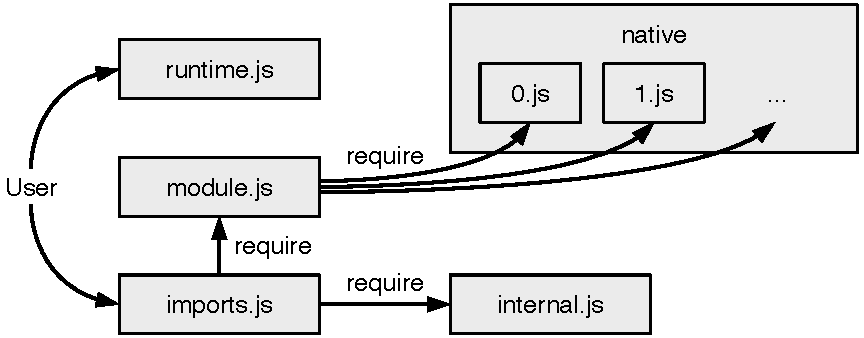
\includegraphics[width=0.8\textwidth]{javaScriptIntegration/bundle}
\end{center}

Auf die praktische Verwendung der JavaScript-Dateien wird in diesem Kapitel nicht eingangen. Im Abschnitt \ref{sec:NodeJSExample} wird anhand eines Beispiels gezeigt, wie sich das Paket in eine Node.js-Konsolenanwendung integrieren lässt.

\section{JavaScript-Codegenerierung}

Wie im vorherigen Abschnitt beschrieben, wird beim Kompilieren JavaScript-Code in der Datei \emph{module.js} generiert.

Beim Erzeugen des Bytecodes wurden bereits für die Stringliterale Speicheradressen (ab 1 beginnend) festgelegt. Daher müssen später zur Laufzeit die Stringliterale in der Reihenfolge der Speicheradressen registriert werden. Dies muss geschehen, bevor das WebAssembly-Modul gestartet wird, da zu diesem Zeitpunkt noch keine Objekte erstellt wurden. So wird garantiert, dass sich die Adressen nicht verschieben.

Außerdem muss für jede Klasse ein Konstruktur generiert werden. Dieser hat die Aufgabe, ein JavaScript-Objekt zu erzeugen, in dem alle Instanzvariablen mit einem (je nach Datentyp) sinnvollen Platzhalterwert initialisiert werden. Außerdem wird der MiniJava-Datentyp mit dem Objekt verknüpft. Die Konstrukturen geben als Rückgabewert die Adresse des erzeugen Objekts zurück.

Da jede Klasse auch Instanzvariablen besitzen kann und WebAssembly nicht direkt auf JavaScript-Objekte zugreifen kann, müssen für diese Getter und Setter erzeugt werden, die diese Aufgabe übernehmen. Die Getter bekommen als Parameter nur die Adresse bzw. Referenz des Objekts und müssen den Wert der Instanzvariable (oder die Adresse wenn die Instanzvariable ein Objekt referenziert) zurückgeben. Ähnlich funktionieren die Setter: Diese bekommen zwei Parameter, die Adresse des Objekts und den Wert des neuen Werts für die Instanzvariable (oder die Adresse, wenn es sich um referenzierte Objekte handelt). Setter haben keinen Rückgabewert.

Die Codegenerierung wird anhand eines überschaubaren Beispiel nun detailliert gezeigt. Nachfolgend sieht man den MiniJava-Code für dieses Beispiel:

\lstinputlisting{src/javaScriptIntegration/Example.minijava}

Aus diesem Code wurde die Datei \emph{module.js} erzeugt:

\lstinputlisting{src/javaScriptIntegration/module.js}

Man sieht am Beginn die zwei Stringliterale (1). Etwas weiter unten ist der Konstruktor, der die Instanzvariablen mit \lstinline{0} und \lstinline{null} initialisiert (2). Bei (3) werden Getter und Setter für die \lstinline{int}-Instanzvariable definiert. Da es sich um einen elementaren Datentyp handelt, kann der Wert direkt aus dem übergebenen Parameter gelesen werden (Setter) bzw. als Rückgabewert zurückgegeben werden (Getter). Beim Getter und Setter für die \lstinline{String}-Instanzvarible (4) muss der Parameter beim Setter zunächst derefenziert werden bzw. muss beim Getter zunächst eine Referenz auf das Objekt erzeugt werden.

\section{Sprachinterne Funktionen}
\subsection{Arrayfunktionen}
\subsection{Stringkonkatenation}

\section{Methodenaufrufe von JavaScript nach MiniJava}

\section{Objektverwaltung für MiniJava in JavaScript}
\subsection{Aufbau}
\subsection{Typinformationen}
\subsection{Hilfsfunktionen}

\section{Auszug aus der Standardbibliothek}

\chapter{Testen des Compilers und Integration des Compilers in Gradle}
\label{cha:Testen-des-Compilers}

\section{Testen}

Über die gesamte Entwicklungsphase des Compilers muss sichergestellt werden, dass beim Hinzufügen neuer Funktionalitäten, diese wie erwartet funktionieren. Gleichzeitig musste auch gewährleistet werden, dass die bereits bestehende Funktionalität des Compilers nicht (versehentlich) verändert wird.

Grundsätzlich stehen zwei Ansätze zum Testen zur Verfügung:
\begin{enumerate}
    \item Jede Komponente isoliert testen, dies entspricht klassischen Unit-Tests. Hier könnte man testen, ob zum Beispiel die erwünschten Instruktionen für eine Schleife generiert werden. 
    \item Testen, ob ein gegebener MiniJava-Quelltext nach dem Kompilieren eine erwartete Konsolenausgabe beim Ausführen produziert. Das entspricht eher einem Integrationstest. Dabei werden in jedem Testfall alle Teilprozesse (Kompilieren, Codegenerieren und Ausführen) ausgeführt.
\end{enumerate}

Es wurde der zweite Ansatz gewählt, da er während des Entwickels eine größere Flexibilität bietet. Die finale Architektur des Compilers entstand erst im Laufe der Entwicklung. Am Anfang war zu erwarten, dass sich interne Strukturen des Compilers laufend ändern könnten. Klassische Unit-Tests müsste man bei größeren Architekturänderungen immer wieder anpassen. Bei Tests, die den gesamten Prozess vom Kompileren bis zum Ausführen als Black-Box betrachten, ist eine Änderung nicht notwendig, da bei den einzigen zwei Schnittstellen (MiniJava-Quelltext und Konsolenausgabe) zwischen Implementierung und Tests keine Änderungen zu erwarten sind. Außerdem bilden alle Testfälle gemeinsam eine Art Spezifikation für die Programmiersprache.

Als Testframework wird JUnit 5 \cite{JUnit} in Kombination mit AssertJ \cite{AssertJ} eingesetzt. Nachfolgend wird ein ein Beispiel für einen einfachen Testfall dargestellt:

\lstinputlisting{src/testenGradle/simpleTest.kt}

Beim Durchführen des Tests wird im Hintergrund eine Datei (\emph{main.minijava}) mit dem zu testenden MiniJava-Quelltext angelegt. JUnit 5 bietet die Annotation \lstinline{@TempDir} an, mit der ein temporäres Verzeichnis für jeden Testfall angelegt wird, das nach Ablauf der Tests wieder gelöscht wird \cite{JUnit}. So werden die Testfälle voneinander isoliert.

Hilfsmethoden wie \lstinline{compileAndRunInMainClass} starten den Compiler und führen das erzeugte Modul aus. Am Ende wird die Konsolenausgabe als Zeichenkette zurückgegeben.

Unter Zuhilfenahme von AssertJ lassen sich die erwarteten Ergebnisse fast wie ein englischer Satz elegant formulieren, zum Beispiel: \lstinline{assertThat(...).containsExactly(...)} \cite{AssertJ}.

Es ist auch möglich, native Methoden auf diese Art zu testen. In diesem Fall wird zusätzlich ein Stück JavaScript-Quelltext mitgegeben. Dieser Quelltext wird in die Datei \emph{main.js} gespeichert, die ebenfalls im temporären Verzeichnis liegt.

Nachfolgend ein einfaches Beispiel für so einen Testfall:

\lstinputlisting{src/testenGradle/nativeTest.kt}

\section{Gradle-Task und -Plugin}
\label{sec:GradleTask-und-Plugin}

Es ist möglich, den MiniJava-Compiler direkt, zum Beispiel über die Kommandozeile, aufzurufen. Für praktische Projekte ist allerdings eine Integration in bestehende Build-Systeme (in diesem Fall Gradle) nützlich, wie es bei anderen Programmiersprachen (zum Beispiel Java und Kotlin) üblich ist.

In der Gradle-Dokumentation \cite{Gradle} wird beschrieben, wie eigene Erweiterungen für Gradle implementiert werden können. Nachfolgend werden die notwendigen Schritte erläutert, die speziell für den MiniJava-Compiler notwendig sind, um ihn in Gradle zu integrieren.

Zunächst wird ein eigener Task (\lstinline{MiniJavaCompilationTask}) definiert, der das Kompilieren von MiniJava-Quelltext kapselt. Dieser Task ist von \lstinline{JavaExec} abgeleitet. Der \lstinline{JavaExec}-Task wird von Gradle zur Verfügung gestellt und kann, ähnlich wie die java-Komman\-dozeile, kompilierte Bytecode-Klassen ausführen. Im \lstinline{MiniJavaCompilationTask} wird der \lstinline{JavaExec}-Task konfiguriert, damit er die Hauptklasse des Compilers (\lstinline{MainKt}) mit den gewünschten Parametern aufruft:

\lstinputlisting{src/testenGradle/MiniJavaCompilationTask.groovy}

Der \lstinline{MiniJavaCompilationTask} bietet zusätzlich noch die Methoden \lstinline{inputDirs} und \lstinline{outputDir} an, mit denen der Task konfiguriert werden kann. Die Methoden speichern die übergebenen Verzeichnisnamen und leiten daraus die Parameter für den Compiler ab (\lstinline{updateArg}). Über \lstinline{inputs.dir(...)} und \lstinline{outputs.dir(...)} können in Gradle Metainformationen für den Task definiert werden, die beschreiben, von welchen Dateien der Task abhängig ist und welche Dateien der Task produziert. So kann Gradle den Build-Prozess optimieren, indem beispielsweise nur dann der MiniJava-Compiler ausgeführt wird, wenn sich eine MiniJava-Quelltext-Datei verändert hat.

Der \lstinline{JavaExec}-Task benötigt zum Ausführen einen Klassenpfad, in dem die MiniJava-Compiler-Klassen enthalten sind. Dieser Klassenpfad hat einen eigenen Namen (\lstinline{project.configurations.minijava}) und ist unabhängig von anderen, die in Gradle definiert sind (wie beispielsweise \lstinline{implementation}, \lstinline{testImplementation} und \lstinline{compileOnly})

Der \lstinline{minijava}-Klassenpfad muss daher zunächst im Gradle-Projekt definiert werden. Dies ist mit Hilfe eines eigenen Plugins möglich:

\lstinputlisting{src/testenGradle/MiniJavaPlugin.groovy}

Damit andere Gradle-Projekte das Plugin finden, gibt es mehrere Möglichkeiten. Bei der hier eingesetzten Variante genügt es, im Gradle-Wurzelprojekt ein Verzeichnis \lstinline{buildSrc} zu erstellen, in dem der Quelltext vom Task und Plugin gemäß folgender Verzeichnisstruktur abgelegt wird:

\lstinputlisting{src/testenGradle/buildSrc.txt}

Weiters ist darin die Datei \emph{dev.ssch.minijava.properties} notwendig, in welcher der Name der Plugin-Klasse definiert wird:

\lstinputlisting{src/testenGradle/dev.ssch.minijava.properties}

\lstinline{dev.ssch.minijava} im Dateinamen dieser Datei ist der Bezeichner, unter dem das Plugin von anderen Gradle-Projekten gefunden werden kann.

\section{Integration von MiniJava in eine Node.js-Konsolenanwendung}
\label{sec:NodeJSExample}

Auf Basis der Vorbereitungen im vorherigen Abschnitt kann der Compiler nun in eigenen Projekten eingesetzt werden. Nachfolgend wird die Konfiguration in Gradle, sowie das Einbinden in eine Node.js-Konsolenanwendung demonstriert.

Die Node.js-Konsolenanwendung ist folgendermaßen strukturiert:

\lstinputlisting{src/testenGradle/demo-nodejs.txt}

In der Datei \emph{build.gradle} wird folgende Konfiguration vorgenommen:

\lstinputlisting{src/testenGradle/build.gradle}

Nachfolgend einige Erklärungen zu \emph{build.gradle}:
\begin{itemize}
    \item In Zeile 5 wird das Plugin mit dem im vorherigen Abschnitt definierten Bezeichner aktiviert.
    \item In Zeile 9 wird der Compiler in den Klassenpfad \lstinline{minijava} gelegt.
    \item In den Zeilen 12 bis 15 wird der vorher definierte Task instanziert und mit zwei Quelltext-Verzeichnissen (Standardbibliothek und das \emph{minijava}-Verzeichnis) und dem Ausgabe-Verzeichnis (\emph{build/wasm-module}) parametrisiert.
\end{itemize}

Die Standardbibliothek befindet sich außerhalb des Projektverzeichnisses, um sie in verschiedenen Projekten wiederverwenden zu können.

In der Datei \emph{index.js} kann nun das kompilierte MiniJava-Modul, wie in Node.js üblich, mit \lstinline{require} importiert und anschließend aufgerufen werden:

\lstinputlisting{src/testenGradle/index.js}

Das Projekt kann nun mit \lstinline{node index.js} gestartet werden.

\vspace{4em}
In diesem Kapitel wurde gezeigt, wie der Compiler getestet werden kann, um die korrekte Funktionalität von diesem sicherzustellen. Weiters wurde gezeigt, wie der Compiler in Gradle integriert werden kann. Die praktische Verwendung davon wurde anhand einer Node.js-Konsolenanwendung demonstriert.

Im nächsten Kapitel wird die praktische Verwendung aller bisherigen Bestandteile im einer abgeschlossenen Web-Anwendung gezeigt.

\chapter{Demo-Anwendung im Browser}
\label{cha:DemoAnwendung}

Um die praktische Anwendung von MiniJava für typische Browser"=Anwendungen zu demonstrieren, wurde eine einfache Web"=Anwendung implementiert, die Fibonacci"=Zahlen berechnen kann.

\section{Anforderungen an den Fibonacci-Rechner}
Die Benutzeroberfläche soll zwei Eingabefelder (für Werte $a$ und $b$) und einen Start"=Knopf darstellen. Beim Drücken des Start"=Knopfs soll die Anwendung die Fibonacci"=Zahlen von $fib(a)$ bis $fib(b)$ berechnen und in einer Tabelle ausgeben.

Der Fokus des Fibonacci"=Rechners liegt darauf, MiniJava in einem abgeschlossenen Projekt zu präsentieren und zu zeigen, wie MiniJava mit dem Browser interagieren kann. Dabei wurde der Aspekt einer effizienten Implementierung bewusst vernachlässigt. Dadurch wirken zwar einige Quelltext"=Abschnitte erzwungen (beispielsweise das rekursive Berechnen jeder einzelnen Fibonacci-Zahl ohne Speichern von Zwischenergebnissen oder das Kapseln von Methodenparametern in Objekte), gleichzeitig wird dadurch aber ermöglicht, im Rahmen eines überschaubaren Anwendungsfalls möglichst viele Funktionalitäten von MiniJava einzusetzen.

Zum Vergleich wurden diesselben Anforderungen zur Gänze auch in JavaScript implementiert. Ziel ist dabei lediglich ein Vergleich zwischen den Programmiersprachen und nicht eine idente oder gar deckungsgleiche Implementierung.

In diesem Kapitel werden nur relevante Quelltext"=Ausschnitte gezeigt. Die vollständige Implementierung findet sich im Git"=Repository.

\pagebreak
\section{Implementierung in MiniJava}

Nachfolgend findet sich die Implementierung des Fibonacci"=Rechners in MiniJava.
\lstinputlisting{src/demoAnwendung/ClickEventListener.minijava}
\pagebreak
\lstinputlisting{src/demoAnwendung/FibonacciCalculator.minijava}
\lstinputlisting{src/demoAnwendung/Main.minijava}

\section{Implementierung in JavaScript}

Nachfolgend findet sich die Implementierung des Fibonacci"=Rechners in JavaScript.
\lstinputlisting{src/demoAnwendung/js-version.js}

\section{Build-Prozess und Ausführen der Web-Anwendung}

Ähnlich wie bei der Konsolenanwendung im vorherigen Kapitel wird hier ebenfalls Gradle eingesetzt, um den MiniJava"=Quelltext zu kompilieren. Zusätzlich dazu wird webpack \cite{Webpack} eingesetzt, um alle JavaScript"=Dateien in eine einzige JavaScript"=Datei zusammenzufassen. Sämtliche \lstinline{require}"=Referenzierungen werden dabei aufgelöst.

Zusätzlich zur Basis"=Standardbibliothek wird eine eigene für den Browser mitkompiliert. Diese enthält Funktionalitäten, die auf Browser"=Schnittstellen abgebildet werden (Implementierungdetails sind im nächsten Abschnitt zu finden).

Beim Ausführen muss sichergestellt werden, dass das binäre WebAssembly"=Modul vom Web"=Server mit dem MIME"=Type \lstinline{application/wasm} bereitgestellt wird, sonst kann es zu Laufzeitfehlern kommen \cite{MDNWebAssembly}. Zu Entwicklungs- und Testzwecken reicht dafür das NPM"=Modul \lstinline{lite-server}\footnote{\url{https://www.npmjs.com/package/lite-server}} vollkommen aus. Für den produktiven Einsatz sollte man diesen Aspekt bei der Konfiguration des Web"=Servers beachten. Im Git"=Repository findet sich eine lauffähige Konfiguration für den Apache HTTP Server in Form eines \emph{Dockerfiles}.

\section{Auszug aus der Standardbibliothek für den Browser}

Um in MiniJava sinnvoll mit dem Browser interagieren zu können, wurde eine kleine Standardbibliothek entwickelt. Zwei Funktion daraus werden nun im Detail betrachtet: Das Abfragen eines HTML"=Knotens aus dem DOM über die ID des Elements und das Hinzufügen eines Event"=Listeners für das Mausklick"=Ereignis zu einem HTML"=Knoten.

\lstinputlisting{src/demoAnwendung/Browser.minijava}
\lstinputlisting{src/demoAnwendung/Browser.js}

Nachfolgend einige Details zum JavaScript"=Teil der beiden Methoden:

Mit der Funktion \lstinline{runtime.wasmRef} können DOM"=Knoten, welche die JavaScript"=Funktion \lstinline{document.getElementById} zurückgibt, MiniJava zugänglich gemacht werden.

Als Event"=Listeners für das Mausklick"=Eregnis wird eine JavaScript"=Funktion (Lambda"=Ausdruck) registriert. Diese Funktion delegiert das Ereignis an das beim Registieren übergebene \lstinline{handler}"=Objekt. Dabei wird angenommen, dass in der Klasse dieses Objekts eine Methode namens \lstinline{handleEvent} existiert, die einen Parameter vom Typ \lstinline{MouseEvent} annimmt. Sollte so eine Methode nicht existieren, kommt es zu einem Laufzeitfehler.

\section{Ergebnis}

In Abbildung \ref{fig:fibCalculatorBrowser} sind zwei Bildschirm"=Schnappschüsse des Fibonacci"=Rechners im Browser. Links wurde die JavaScript"=Version ausgeführt, rechts die MiniJava"=Version. Man erkennt bei den ersten Zahlen, dass diese korrekt berechnet wurden.

\begin{figure}[]
    \centering
    \begin{tabular}{c c}
        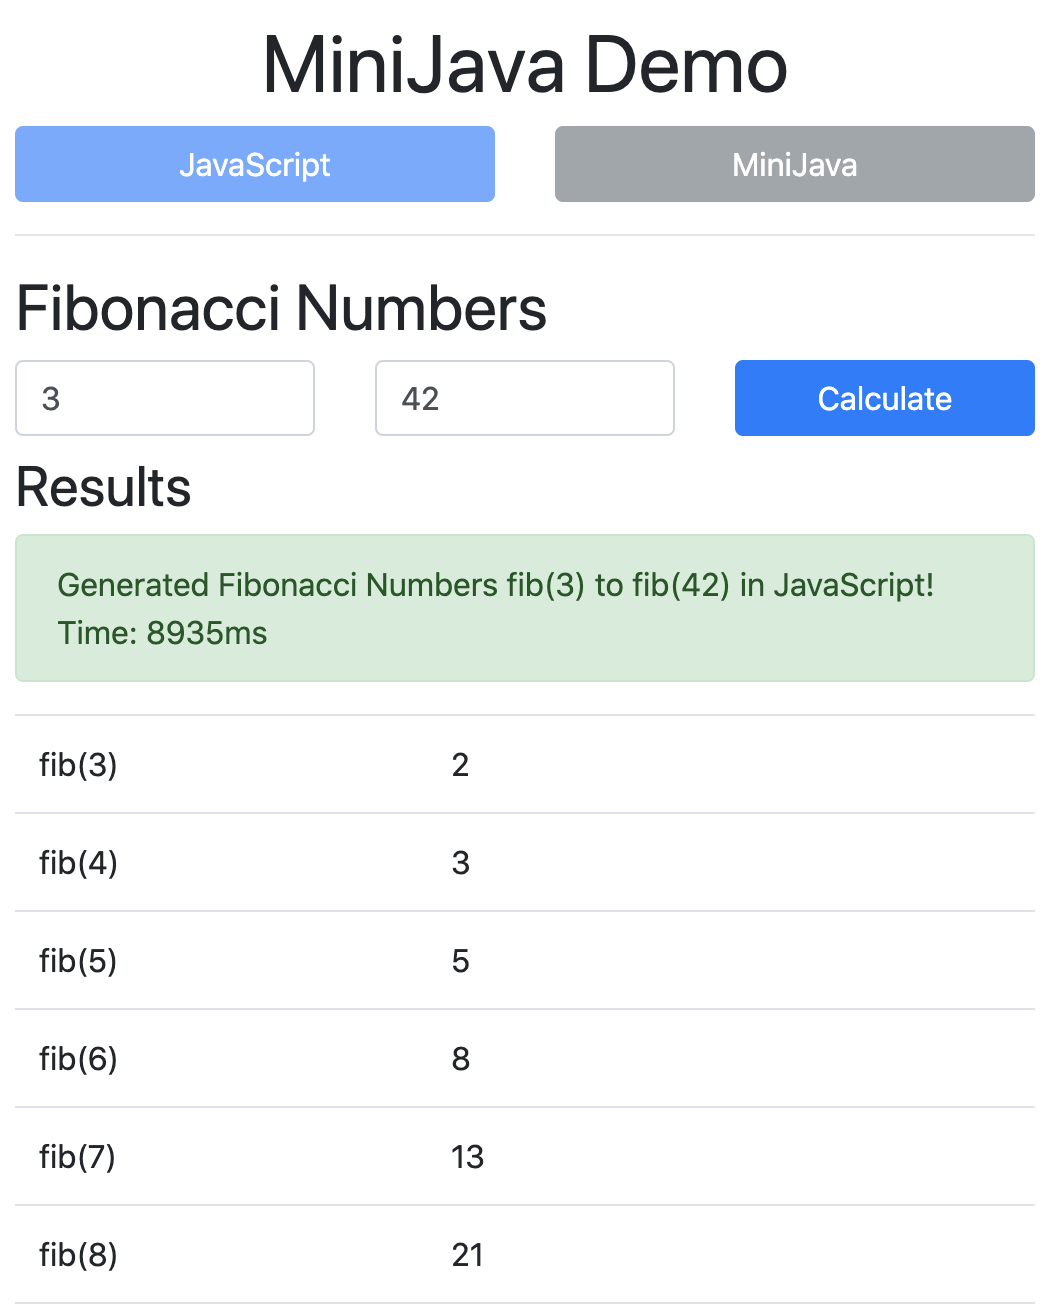
\includegraphics[width=0.47\textwidth]{demoAnwendung/fibonacciJavaScript} & 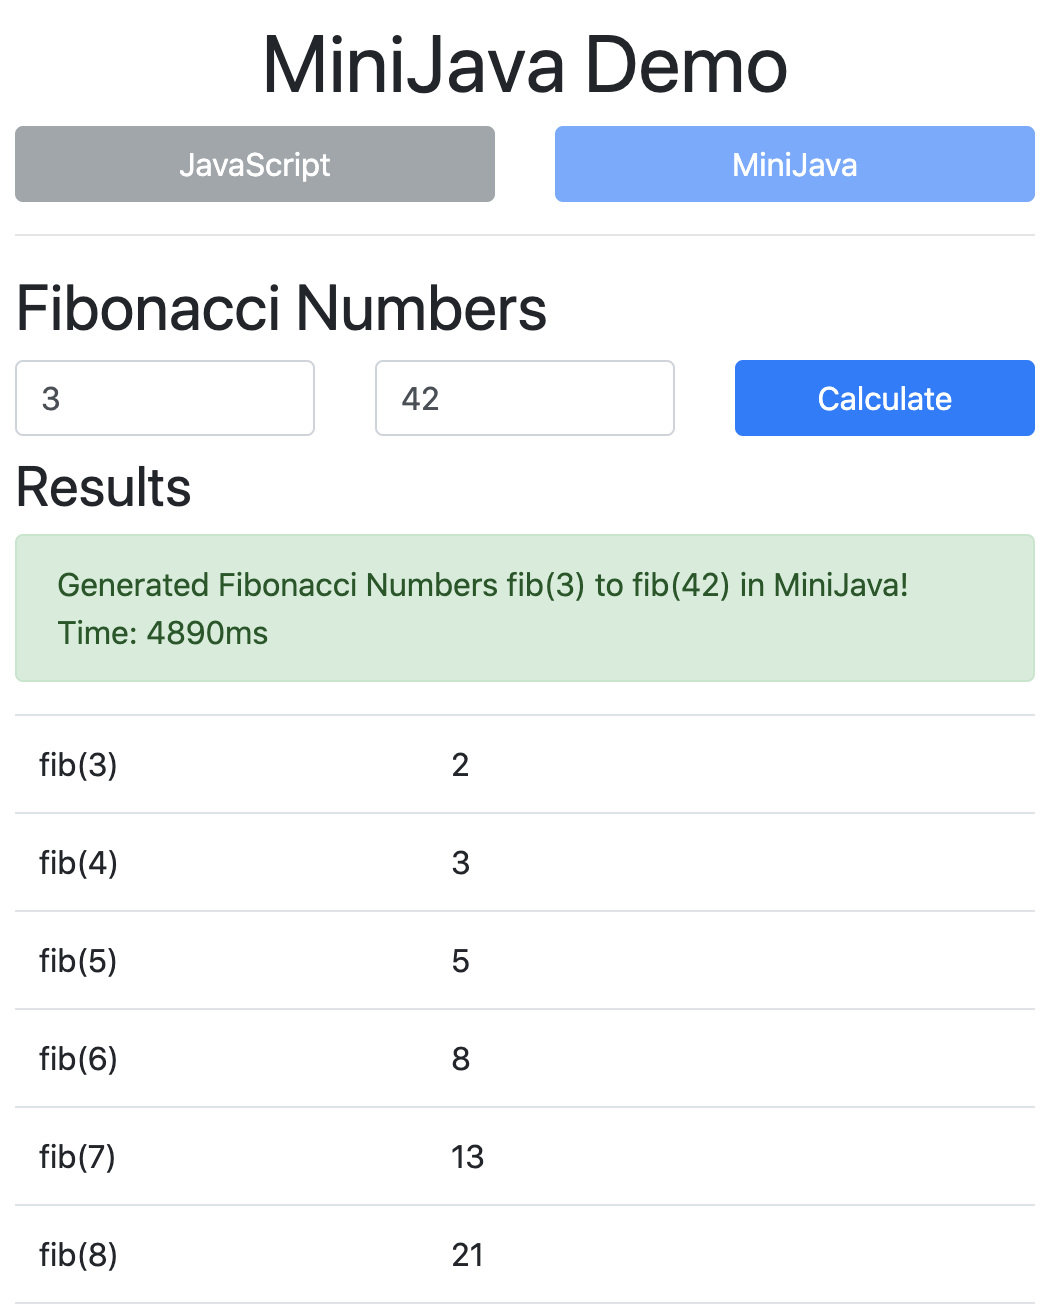
\includegraphics[width=0.47\textwidth]{demoAnwendung/fibonacciMiniJava}
    \end{tabular}
    \caption{Fibonacci-Rechner im Browser}
    \label{fig:fibCalculatorBrowser}
\end{figure}

Während der Ausführung wurde die Laufzeit gemessen, dabei wird die gesamte Zeit ab dem Klicken des Start"=Knopfs bis zum Erstellen der Tabelle berücksichtigt. Man erkennt, dass die Laufzeit der MiniJava"=Version (4890 Millisekunden) im Vergleich zur JavaScript"=Version (8935 Millisekunden) deutlich kürzer ist.

Der Fibonacci"=Rechner wurde auf der folgenden Sofware- und Hardware"=Konfiguration getestet:
\begin{itemize}
    \item Browser: Google Chrome (Mac) 81.0.4044.122 64"=Bit
    \item Betriebssystem: macOS 10.15.4
    \item Hardware: MacBook Pro (15"=inch, 2018)
    \begin{itemize}
        \item CPU: 2,6 GHz 6"=Core Intel Core i7
        \item RAM: 16 GB 2400 MHz DDR4
    \end{itemize}
\end{itemize}

\section{Vergleich JavaScript und MiniJava}

Insgesamt sieht, man dass die Implementierungen aus Quelltextsicht sehr ähnlich sind. Sämtliche Anforderungen wurden von beiden Varianten erfüllt.

Die Quelltextmenge ist bei JavaScript deutlich geringer, da keine Datentypen deklariert werden müssen, sondern diese direkt verwendet werden können. Außerdem bietet JavaScript im Vergleich zu MiniJava mehr syntaktische Konstrukte wie beispielsweise die \lstinline{for}"=Schleife oder Lambda"=Ausdrücke. 

Der wesentliche Vorteil bei MiniJava ist die Typsicherheit, da sämtliche Zugriffe auf Objekte bereits beim Kompilieren überprüft werden und beispielsweise flüchtige Tippfehler früh erkannt werden. Bei der Typsicherheit gibt es eine einzige Ausnahme: das Aufrufen der \lstinline{handleEvent}"=Methode, da von der Standardbibliothek angenommen wird, dass diese Methode existiert. Würde man allerdings MiniJava um \emph{Interfaces} erweitern, könnte man dieses Problem lösen, da dann wieder der Compiler in der Lage wäre, die Anwesenheit von Methoden zu garantieren.

Anhand der Laufzeitmessungen sieht man, dass die MiniJava"=Variante deutlich schneller läuft. Dies ist vor allem auf den rechenintensivsten Teil, der rekursiven Berechnung für jede einzelne Zahl, des Programms zurückzuführen, der bei MiniJava ausschließlich in der virtuellen WebAssembly"=Maschine läuft. Die Laufzeiten verhielten sich über mehrere Aufrufe hintereinander bei beiden Varianten stabil.

\vspace{4em}
In diesem Kapitel wurde der praktische Einsatz von MiniJava anhand des Fibonacci"=Rechners demonstriert. Es wurde ebenfalls auf den Build"=Prozess und die Interaktion mit dem Browser eingangen. Dieselbe Anwendung wurde ebenfalls mit JavaScript implementiert. Die beiden Implementierungen wurden miteinander verglichen.

\chapter{Zusammenfassung}

In diesem Kapitel werden die Ergebnisse der Arbeit zusammengefasst und es wird ein Ausblick auf mögliche Erweiterungen des MiniJava-Compilers und alternative Ansätze gegeben. Zum Schluss gebe ich einen Einblick auf meine persönlichen Erfahrungen während der Entwicklung des Compilers.

\section{Ergebnisse}

Alle vier Fragen der Problemstellung wurden in dieser Arbeit beantwortet:
\begin{enumerate}
	\item Was ist WebAssembly, welche Möglichkeiten bietet WebAssembly und welche Einschränkungen gibt es?
	\item Wie kann ein Compiler, der eine Programmiersprache nach WebAssembly übersetzt, implementiert und getestet werden?
	\item Wie werden typische Sprachkonstrukte einer Programmiersprache auf Web\-Assem\-bly-Befehle abgebildet?
	\item Wie wird die Schnittstelle zum Browser entworfen und auf welche Aspekte muss dabei geachtet werden?
\end{enumerate}

Zu Beginn wurde im \ref{cha:Technische-Grundlagen} Kapitel (Technischen Grundlagen) WebAssembly als Technologie detailliert behandelt. Weiters wurden drei Technolgien (Emscripten, Rust und Blazor) vorgestellt, die bereits auf WebAssembly aufbauen. Dabei wurden auch einige Einschränkungen von WebAssembly dargestellt, beispielsweise kann nicht zu jeder beliebigen Instruktion gesprungen werden, da Sprünge strukturiert sein müssen. Weiters wurde ein Ausblick auf weitere Entwicklungen von WebAssembly gegeben. In den technischen Grundlagen wurden außerdem diverse Technologien behandelt, die für die Implementierung notwendig sind, wie beispielsweise ANTLR und Kotlin. Hier wurde die erste Frage der Problemstellung beantwortet

In Kapitel \ref{cha:MiniJava} wurde die Programmiersprache MiniJava vorgestellt, für die ein Compiler entwickelt wurde. Weiters wurde auf die Anforderungen an das Laufzeitsystem eingegangen.

Die zweite Frage wurde in den Kapiteln \ref{cha:Codegenerierung-für-WebAssembly} und \ref{cha:Testen-des-Compilers} beantwortet. Hier wurde gezeigt, wie die Sprachkonstrukte aus MiniJava auf WebAssembly-Bytecode abgebildet werden und wie der Compiler getestet wird. JavaScript-Aspekte, die zur Laufzeit notwendig sind, wurden in Kapitel \ref{cha:JavaScript-Integration} dargestellt. Dazu zählt beispielsweise die Objektverwaltung.

Zum Schluss wurde die Funktionalität des gesamten Systems anhand einer Demo-Anwendung, dem Fibonacci-Rechner, in Kapitel \ref{cha:DemoAnwendung} gezeigt. Weiters wurde Frage 4 mit einem Einblick in die Standardbibliothek für Browser-Zugriffe beantwortet. Der Zugriff erfolgt über native Methoden, die in MiniJava aufgerufen werden können, deren Implementierung aber in JavaScript hinterlegt ist.

Alle Vorhaben wurden umgesetzt und die Implementierung des Compilers ist gelungen. MiniJava kann in eigenen Projekten für Browser-Anwendungen eingesetzt werden. Die Integration in bestehende Systeme ist ebenfalls möglich.

\section{Ausblick}

Während dem Erstellen der gesamten Arbeit sind einige interessante Ideen und Ansätze entstanden, die aber leider nicht umgesetzt wurden, da sie schlicht und einfach den Rahmen der Arbeit gesprengt hätten. Nachfolgend findet sich eine Liste all dieser Ideen und Ansätze:
\begin{itemize}
    \item Bessere Integration des Garbage-Collectors: Derzeit werden alle in MiniJava verwendete Objekte in einer JavaScript-Datenstruktur verwaltet. Die Objete bleiben jedoch in dieser Datenstruktur enthalten, auch wenn sie in nirgends mehr benötigt werden. Sie verbrauchen dadurch unnötig Ressourcen. JavaScript bietet mit einem eigenen Garbage-Collector bereits Fuktionalitäten an, nicht mehr benötigte Ressourcen freizugeben. Diesen könnte man besser integrieren, um die Ressourcennutzung zu optimieren.
    \item Den gesamten Java-Sprachumfang unterstützen: MiniJava fehlen Funktionalitäten, die in Java enthalten sind, dazu zählen beispielsweise \emph{vollständige Objektorientierung}, dynamische Bindung von Methoden zur Laufzeit, Lambda-Ausdrücke, \emph{Interfaces}. Für all diese Funktionalitäten müsste man entsprechende Abbildungen in WebAssembly finden. Dadurch könnte man schlussendlich im Idealfall auch einen Großteil der Java-Standardbibliothek im Browser einsetzen.
    \item MiniJava-Objekte im WebAssembly-Speicher: Ursprünglich wurden im ersten Entwurf alle MiniJava-Objekte im WebAssembly-Speicher abgelegt. Dieser wurde aber wieder verworfen, da durch die Abbildung auf JavaScript-Objekte der Zugriff auf den DOM signifikant vereinfacht wurde. Aus Performanzsicht wäre es eine Überlegung, dennoch einige Objekte im WebAssembly-Speicher zu verwalten, wenn sie nur MiniJava-intern verwendet werden. Eine einfache Möglichkeit wäre, eine Klasse mit einer eigenen Annotation zu markieren, damit Objekte dieser Klasse nicht mehr auf JavaScript abgebildet werden, sondern im WebAssembly-Speicher abgelegt werden. So könnte man je nach Anwendungsfall zwischen den beiden Möglichkeiten wählen.
    \item Java-Bytecode konvertieren: Anstatt den gesamten Compiler neu zu erfinden, könnte man versuchen, Java-Bytecode direkt in WebAssembly-Bytecode abzubilden. Da die JVM ebenfalls mit einem Kellerspeicher arbeitet, wären einige Aspekte direkt abbildbar. Andere Aspekte müsste man etwas aufwendiger konvertieren, dazu gehören beispielsweise Sprünge zu beliebigen Instruktionen, die so nicht in WebAssembly möglich sind.
    \item Performanz der virtuellen WebAssembly-Maschine: WebAssembly verspricht hohe Performanz. Im Fibonacci-Rechner dieser Arbeit scheint die WebAssembly-Variante schneller zu sein, dies wurde aber nicht genauer erforscht. Daher wären umfangreiche Performanzmessungen interessant, um herauszufinden, um wie viel \emph{besser} WebAssembly im Vergleich zu reinem JavaScript abschneidet.
    \item Testen ausweiten und verbessern: Die Funkionalität des Compilers wurde mit einer großen Menge an Testfällen (zum Zeitpunkt der Fertigstellung der Arbeit über 350) validiert. Sie decken jede Sprachfunktionalität ab und waren eine große Hilfe bei größeren Architekturänderungen und Refactorings. Da Sprache MiniJava ist unendlich groß, daher können unmöglich alle Randfälle abgedeckt werden. Um daher zumindest den Testumfang zu vergrößeren, wäre das automatische Generieren von Testfällen nützlich. Eine Möglichkeit solche Testfälle zu erzeugen, wäre das \emph{zufällige} Erzeugen von MiniJava-Quelltext basierend auf der Grammatik. Um das erwartete Ergebnis dieses Quelltexts zu erhalten, könnte man ihn mit dem Java-Compiler kompilieren und ausführen.
    \item Zukünftig ist es vielleicht nicht mehr notwendig, gewisse Funktionalitäten, wie beispielsweisen den Zugriff auf JavaScript-Objekte, händisch nachzubauen. WebAssembly ist eine aktiv wachsende Technologie und könnte daher zukünftig solche Funktionalitäten selbst enthalten.
\end{itemize}

\section{Persönliche Erfahrung}

Mir hat das Erstellen eines neuen Compilers einschließlich der gesamten Workflow bis zur Laufzeit sehr viel Spaß gemacht und hat mir noch bessere Einblicke in die Komplexität des Compilerbaus gegeben. Im 2. Bachelorsemester und 1. Mastersemester Software Engineering wird das Thema Compilerbau in eigenen Lehrveranstaltungen am Beispiel von Untermengen von Pascal, C und C++ behandelt. Diese Grundlagen waren mehr als ausreichend, um den MiniJava-Compiler zu entwickeln. Da der Sprachumfang von MiniJava jedoch sehr umfangreich, war die Architektur und sauberere Strukturierung des Compilers selbst eine neue Herausforderung. Daher war es die richtige Entscheidung von Anfang an auf Testgetriebene Entwicklung zu setzen, um Architekturanpassungen im Laufe der Zeit zuverlässig (und ohne große Sorge, \emph{dass etwas kaputt geht}) umsetzen zu können. WebAssembly hat ein großes Potenzial und bleibt in den nächsten Jahren eine spannende Entwicklung, die es zu beobachten gilt, vor allem, da WebAssembly mittlerweile ein Standard des W3C ist. Besonders interessant werden die zukünftigen Erweiterungen und die Verwendung von WebAssembly, da sich WebAssembly auf sehr unterschiedliche Arten (wie man bei Emscripten, Rust, Blazor und MiniJava sieht) einsetzen lässt.


%%%----------------------------------------------------------
\appendix                                            % Anhang 
%%%----------------------------------------------------------

\chapter{MiniJava-Grammatik in ANTLR-Syntax}
\label{app:MiniJava-Grammatik}

\lstinputlisting{src/miniJavaGrammatik/MiniJava.g4}


%%%----------------------------------------------------------
\MakeBibliography                        % Quellenverzeichnis
%%%----------------------------------------------------------

%%% Messbox zur Druckkontrolle ------------------------------
\chapter*{Messbox zur Druckkontrolle}



\begin{center}
{\Large --- Druckgröße kontrollieren! ---}

\bigskip

\calibrationbox{100}{50} % Angabe der Breite/Hoehe in mm

\bigskip

{\Large --- Diese Seite nach dem Druck entfernen! ---}

\end{center}



%%%----------------------------------------------------------
\end{document}
%%%----------------------------------------------------------